\section{Fundamentals}
\subsection{Bin Picking}
\subsubsection{Definition and Application}
Bin picking is a robotics and automation technique used in manufacturing and logistics, automotive industry, particularly in warehouses and assembly lines. It involves locating, grabbing and manipulating objects from a bin or container utilizing robotic devices equipped with sensors, cameras and algorithms. Thus, it is a crucial area of interest for research in computer vision and robotics. There are usually multiple steps in the process: sensing and perception, planning and path calculation, grasping and manipulation, ultimately transportation and placement which will be further elaborated in the following passages.\cite{bin_picking}

\vspace{5mm}

\textbf{Sensing and Perception} To determine the kind position orientation and the kind of objects inside a bin or container, the robot uses its sensors and cameras to scan it. For the purpose of identifying the items, especially ones that are partially occluded or organized randomly or have entanglement in between them, advanced computer vision algorithms are used for the purpose.\cite{bin_picking}

\vspace{5mm}

\textbf{Planning and Path Calculation} Following the identification of the items in the bin, the robots control system determines the best course for the arm or gripper to take in order to reach and retrieve the intended item in the bin. Avoiding collision with other objects in the bin and calculating the most efficient path for carrying the objects from one point to another are the two crucial parts in this stage. \cite{bin_picking}
\vspace{5mm}

\textbf{Grasping and Manipulation} The robot can places its arm in a suitable location and employs its gripper to firmly hold the object of interest. Firm and control over the grippers is crucial for this stage to prevent damage and unwanted slippage.\cite{bin_picking}

\vspace{5mm}

\textbf{Transportation and Placement} Once the robot has a firm grip on the object it moves the item to the intended spot, like a shipping container, assembly line or conveyor belt. Before settings the object down, the robot occasionally needs to realign or orient it.\cite{bin_picking}

There are numerous benefits of bin picking in manufacturing and logistics.
\begin{itemize}
  \item \textbf{Enhanced Efficiency} Businesses can greatly boost productivity and throughput, particularly in high-volume operations, by automating the process of selecting goods from bins.
  \item \textbf{Flexibility} Bin picking applications are appropriate for a variety of manufacturing situations because they can handle a wide range of items based on their shapes, size and materials.
  \item \textbf{Savings} Automating manual labor-intensive jobs, such as bin picking, can save labor costs and lower the chance of accidents that come with physical handling.
  \item \textbf{Health of Employees} Picking heavy objects for a longer period of time can often be detrimental for the worker's health. Thus, using automated bin picking solutions can be extremely helpful in such cases.
\end{itemize}
Keeping everything in mind, bin picking applications are essential to contemporary manufacturing and logistic operations, helping businesses to increase productivity and streamline workflows.
\subsubsection{Gripper Types}
Grippers are crucial parts of robotic systems used in bin picking applications that allow them to grab and move objects out of the bins or containers. There are different kinds of grippers and each is appropriate for a particular purpose depending on the shape, size, weight and substance of the objects being handled. The following are a few typical gripper kinds used for bin picking.

\vspace{5mm}

\textbf{Vacuum Grippers} These grippers cling to smooth or flat  surfaces using suction as shown in Fig. \ref{fig:vacuum_gripper}.
\begin{figure}
  \centering
  \begin{minipage}[t]{.45\textwidth}
    \centering
    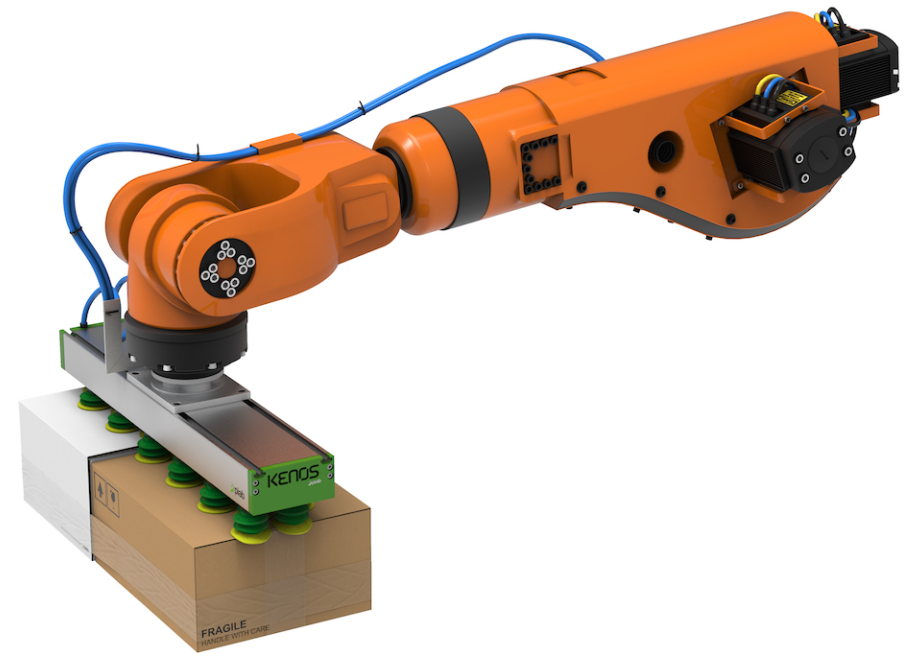
\includegraphics[width=150pt,height=150pt]{pictures/vacuum_gripper.png}
    \captionof{figure}{Vacuum Grippers\cite{vacuum_gripper}}
    \label{fig:vacuum_gripper}
  \end{minipage}%
  \hspace{1cm}
  \begin{minipage}[t]{.45\textwidth}
    \centering
    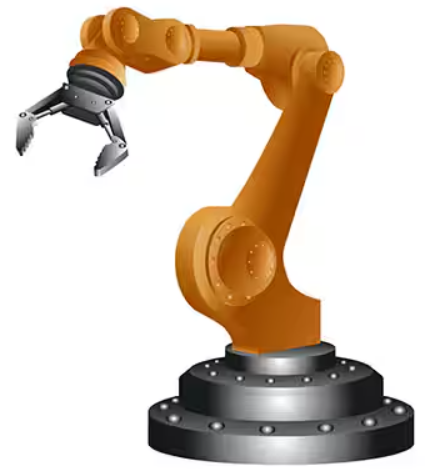
\includegraphics[width=150pt,height=150pt]{pictures/mechanical_gripper.png}
    \captionof{figure}{Mechanical Grippers\cite{mechanical_gripper}}
    \label{fig:mechanical_gripper}
  \end{minipage}
\end{figure}
When handling huge, flat good like sheets of plastic, glass or metal, they are especially useful. By using interchangeable suction cups or pads, vacuum grippers can be made to handle objects of various sizes and shapes. The primary advantage of these type of grippers is the need for one-surface accessibility. This makes handling cluttered bins easier. The drawback however is that a vacuum gripper can still generate traction even if the intended grasping position is not met. This results in a possibly erroneous placement and an imprecise position of the gripper.\cite{spenrath2022heuristic}

\vspace{5mm}

\textbf{Mechanical Grippers} To grasp objects, mechanical grippers use mechanical jaws, fingers or claws. They may be tailored with various jaw configurations to meet particular object geometries and are appropriate for a broad variety of shapes and sizes. Mechanical grippers are useful for picking up objects with uneven shapes, such as bottles, crates and components, as they offer a solid hold as shown in Fig. \ref{fig:mechanical_gripper}. But because of the tough and rigid mechanical nature of the gripper, it might cause damage while handling delicate and sensitive objects.\cite{fager2020gripper}

\vspace{5mm}

\textbf{Magnetic Grippers} These devices draw in and hold onto ferromagnetic materials like steel using electromagnetic forces as shown in Fig. \ref{fig:magnetic_gripper}.
\begin{figure}
  \centering
  \begin{minipage}[t]{.45\textwidth}
    \centering
    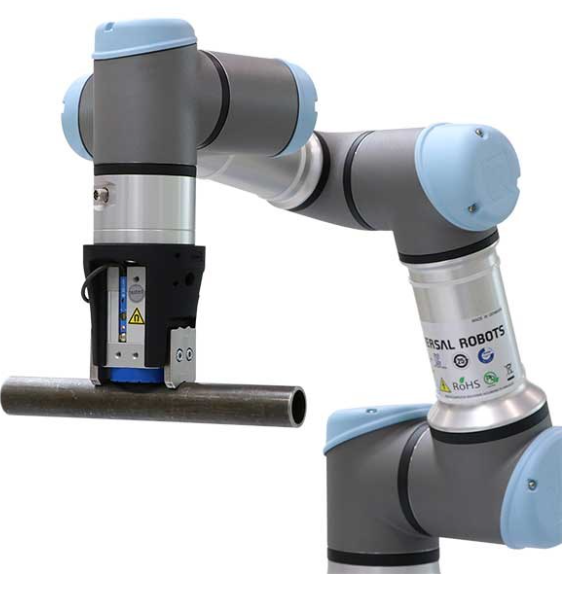
\includegraphics[width=150pt,height=150pt]{pictures/magnetic_gripper.PNG}
    \captionof{figure}{Magnetic Grippers\cite{magnetic_gripper}}
    \label{fig:magnetic_gripper}
  \end{minipage}%
  \hspace{1cm}
  \begin{minipage}[t]{.45\textwidth}
    \centering
    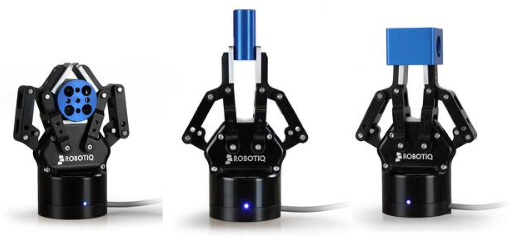
\includegraphics[width=200pt,height=100pt]{pictures/adaptive_gripper.PNG}
    \captionof{figure}{Adaptive Grippers\cite{adaptive_gripper}}
    \label{fig:adaptive_gripper}
  \end{minipage}
\end{figure}
As such, the benefits and drawbacks are similar to those of vacuum grippers. They are appropriate for applications where cleanliness or delicate surfaces are a concern since they are perfect for handling metallic objects without the need for direct contact. Because of its magnetic properties, it can induce magnetic behavior to the objects being handled which is not desirable and can have serious implication in certain applications\cite{spenrath2022heuristic}. Furthermore, it is possible that the gripper might grab multiple objects at a time instead of a single object which is not desirable.\cite{spenrath2022heuristic} 

\vspace{5mm}

\textbf{Adaptive Grippers} These grippers can handle a broad range of sizes and forms without the need for exact placement since they are made to conform to the shape of the object being held as shown in Fig. \ref{fig:adaptive_gripper}. These grippers frequently modify their shape to fit the curves of the object by using inflated bladders or flexible  polymers. However, to facilitate its adaptive property, it demands for complex control algorithms for precise grasping.\cite{park2018hybrid}

\vspace{5mm}

\textbf{Soft Grippers} Designed to softly grab delicate or unusually shaped objects without causing damage, soft grippers are created from responsive materials like silicone or rubber as shown in Fig. \ref{fig:soft_gripper}. 
\begin{figure}
  \centering
  \begin{minipage}[t]{.45\textwidth}
    \centering
    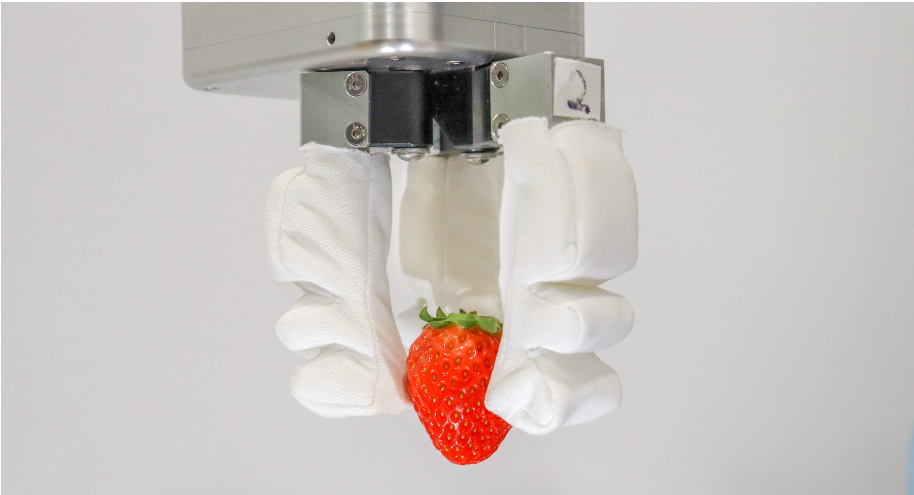
\includegraphics[width=170pt,height=120pt]{pictures/soft_gripper.PNG}
    \captionof{figure}{Soft Grippers\cite{soft_gripper}}
    \label{fig:soft_gripper}
  \end{minipage}%
  \hspace{1cm}
  \begin{minipage}[t]{.45\textwidth}
    \centering
    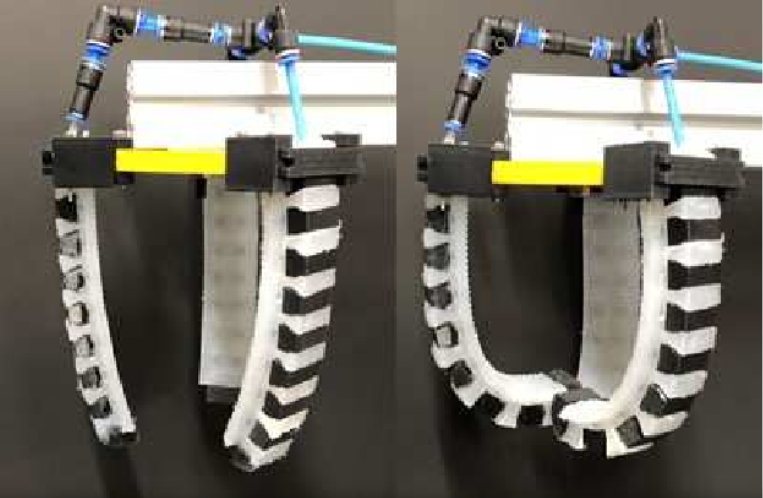
\includegraphics[width=170pt,height=120pt]{pictures/hybrid_grippers.PNG}
    \captionof{figure}{Hybrid Grippers with soft and rigid structures\cite{park2018hybrid}}
    \label{fig:hybrid_gripper}
  \end{minipage}
\end{figure}
They are frequently employed in tasks like picking up food or electrical components, where dexterity and delicate handling are crucial. However, they have lower gripping force as compared rigid grippers, thus, limiting suitability for heavier objects.\cite{park2018hybrid} 

\vspace{5mm}

\textbf{Hybrid Grippers} To improve performance and versatility, hybrid grippers integrate many grasping techniques such as vacuum suctions and mechanical clamping. These grippers are frequently employed in intricate bin picking scenarios where a solitary gripping technique would not be adequate. It also requires more calibration and maintenance due to the integration of multiple systems. It also leads to greater power consumption and computational overhead for executing hybrid gripping mechanism. Thus, the characteristics of the objects being handled, the capabilities of the robotic system and the particular requirements of the application all play a role in the gripper selection. Stakeholders can maximize the effectiveness, dependability and precision of their bin picking processes by choosing the right kind of gripper.\cite{park2018hybrid} 

\subsubsection{Model-Based Approaches}
Model-based  bin picking approaches use a digital model or representation, of the items in the bin as a guide for organizing and carrying out the bin picking procedure. To enable accurate perception and manipulation, these methods make use of \ac{CAD} data or 3-D models of the items. Fig. \ref{fig:model_based} 
\begin{figure}[t]
  \centering
  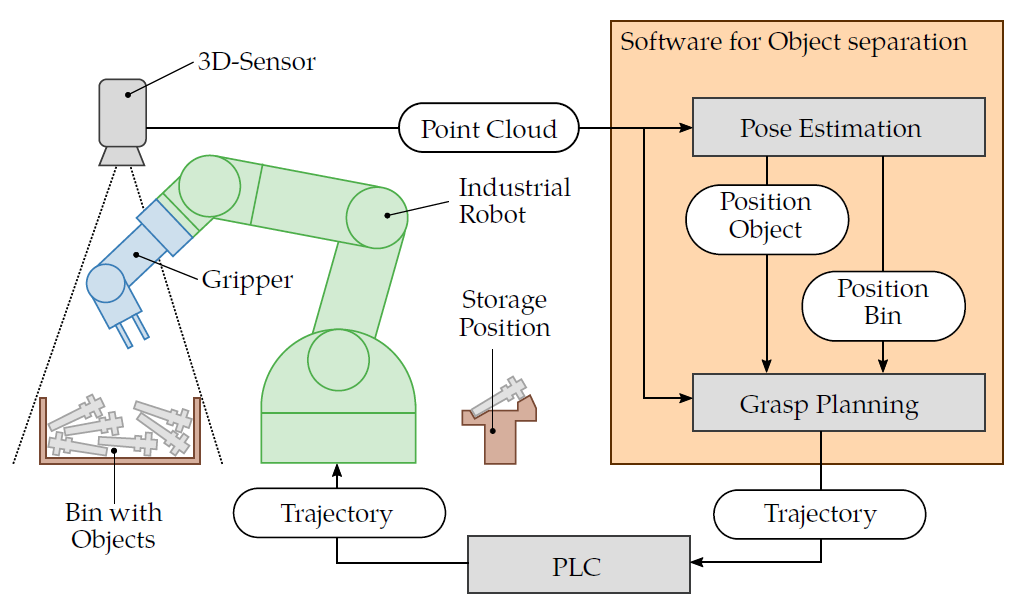
\includegraphics[width=400pt,height=250pt]{pictures/model_based.PNG}
  \caption{Overview of model-based bin picking approach.\cite{spenrath2022heuristic}}
  \label{fig:model_based}
\end{figure}
gives an overview of model-based bin picking approach, an elaboration of which is provided below.

\vspace{5mm}

\textbf{Object Modelling} Creating precise digital models of the objects to be picked is the first stage in a model-based bin-picking strategy. \ac{CAD} software or 3D point cloud generated from real objects through scanning methods like laser scanning or photogrammetry can be used for this. The model ought to be accurately represent the objects surface features, size and geometry.\cite{lin2020robotic}

\vspace{5mm}

\textbf{Bin Perception} The robots sensors, including depth cameras or laser scanners, record information about the contents of the bin once the object models are accessible. Based on the shape, size and orientation of each object in the bin, this data is processed to identify and segment each of them. In order to match and align the perceived objects with their corresponding models, the digital models are used as reference templates.\cite{lin2020robotic}

\vspace{5mm}

\textbf{Pose Estimation} It is the process of figuring out each recognized object's exact location and orientation with respect to the gripper or end effector of the robot. Planning precise gripping trajectories and guaranteeing successful object manipulation depend on this phase. Pose estimation methods include geometric fitting algorithms, point cloud registration and feature mapping.\cite{lin2020robotic}

\vspace{5mm}

\textbf{Grasping Planning} Once the posture of the object is determined, the robot arranges its arm to grasp the object from the bin. In order for the robot's arm or gripper to approach, grasp and safely lift each object, collision-free motion path needs to be calculated. To enable successful gripping, planning algorithms take into account variables including gripper kinematics, object geometry and workspace limitations.\cite{lin2020robotic}

\vspace{5mm}

\textbf{Feedback Control} To monitor and modify the robot's movements in real-time while it is grasping, feedbacks from the sensors such as force/torque sensors or vision systems is utilized. By using feedback control approaches, the robot may adjust its grip in response to unforeseen disruptions or changes in the surroundings, guaranteeing dependable and durable picking performance.\cite{lin2020robotic}

\vspace{5mm}

\textbf{Validation and Verification} The system compares the actual results with the predicted result based on model-based planning to determine whether the grasp was successful after selecting each object. Verifying grasp stability, item alignment and adherence to quality standards are a few examples of validation tasks. The robot can rectify any mistakes by trying to pick the object again or modifying its approach.\cite{lin2020robotic}

\subsubsection{Model-Free Approaches}
The goal of model-free bin picking approach is to pick objects from a bin without using \ac{CAD} data or predefined object models. To identify and handle objects based solely on sensor data, these methods use advanced machine learning algorithms and complex perception techniques. Model-free approaches can be broadly categorized into two groups: deep-learning based approach\cite{bousmalis2018using}, reinforcement learning based approach\cite{levine2018learning} and hybrid perception-based approach\cite{jang2018grasp2vec}. 

\vspace{5mm}

\textbf{Deep Learning-Based Approach} Without explicitly modelling the objects, deep learning techniques like \ac{CNN}s are trained on massive amount of sensor data to learn object recognition and grasping policies on their own. Labelled object instances and corresponding grasping actions are collected from large datasets of sensor data (e.g. \ac{RGB} images, depth maps). Using end-to-end optimization, \ac{CNN}s are trained on those data to acquire grasping policies and object representations. Based on sensor input, robotic systems with trained models are able to grasp objects and identify them in real-time. To enhance grip execution and boost performance, feedback from sensors (such as force/torque sensors) are employed.\cite{bousmalis2018using}

\vspace{5mm}

\textbf{Reinforcement Learning-Based Approach} Without explicit object models, robots can acquire grasping policies through trial and error interactions with the environment by using \ac{RL} techniques. By performing grasping movements and getting feedback (like reward signals) when a task is completed successfully, the robot interacts with its surroundings(e.g. a bin). \ac{RL} algorithms learn grasping policies by optimizing the total rewards earned from the accomplished grasps and interactions with the surroundings. In order to maximize the performance, \ac{RL} agents strike a balance between exploring novel grasping tactics and utilizing previously learnt rules. Robotic systems are equipped with capability to perform bin-picking tasks in real-time.\cite{levine2018learning}

\vspace{5mm}

\textbf{Hybrid Perception-Based Approach} Robots can learn grasping rules from data by combining perception and action primitives in hybrid techniques, which also incorporate domain knowledge or limitations. Using deep learning models or conventional computer vision approaches, sensor data (e.g. \ac{RGB} images) is processed to extract object representation or features. A combination of  imitation learning and reinforcement learning is used to learn grasping policies. Using the learnt policies and the sensor data, perception and action modules work together to optimize the grasping performance. The learnt policies are improved over time by adjusting the grip execution based real-time data from sensors.\cite{jang2018grasp2vec} 

\subsubsection{Robot System}
For pick and place tasks, delta robots and parallel kinematics are the usual system. For bin-picking applications, however, serial kinematics and articulated robots are the more popular options. The advantages include, a much bigger workspace, more degrees of freedom for the end-effector or gripper, allowing a wider range of gripping poses and less limitations sue to internal collisions. The robot system's main task is to match various positions. The following are the three crucial ones for bin picking systems.\cite{spenrath2022heuristic}
\begin{itemize}
  \item The position of the object $\mathbf{W_{P_O}}$ characterizes the object's position in relation to the world coordinates.
  \item The position of the gripper $\mathbf{W_{P_G}}$ characterizes the end-effector's position in relation to the world coordinates.
  \item The grasping position $\mathbf{G_{P_O}}$ characterizes the position of the object in relation to the position of the gripper. This is particularly crucial foe the object's precise placement. 
\end{itemize}
These three positions constitute the closed transformation chain. In other words, the computation of the third pose is easy if the first two are known. These three poses are shown in Fig. \ref{fig:robot_workspace}
\begin{figure}[t]
  \centering
  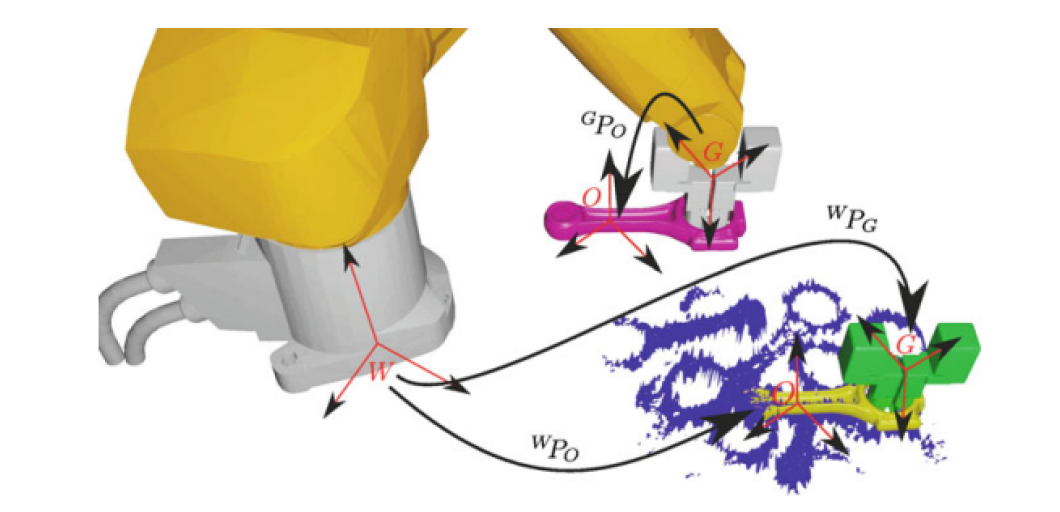
\includegraphics[width=400pt,height=250pt]{pictures/robot_pose.PNG}
  \caption{Important positions of the workspace in a  bin-picking application. $W$ is the world coordinate system with its origin at the centre of the base of the robot. $O$ is the object coordinate system with its origin at the center of the object. $G$ is the gripper coordinate system with its origin at the center of the gripper.\cite{buchholz2015bin}}
  \label{fig:robot_workspace}
\end{figure}
A robot can place its end-effector using one of the two movement techniques: \ac{LIN} motion and \ac{PTP} motion. Every robot motor moves synchronously when in \ac{PTP} motion. Generally speaking, figuring out the trajectory of the \ac{TCP} is difficult when in this mode. The benefit of this motion, however, is its potential to achieve maximum speed. Because of this, this mode is employed to travel great distances between certain poses. The \ac{TCP} is a crucial point in the \ac{LIN} motion. In this motion, the \ac{TCP} travels linearly from one place to another in Cartesian space. Its speed is much slower than in \ac{PTP}, which is a drawback for confined workspaces. Inverse kinematics calculation and singularity avoidance are the two components of the \ac{LIN} mode operation. These configurations are typically detected by robot controller, which will stop the robot.\cite{spenrath2022heuristic}

\subsection{Deep learning-based 3D Image processing}
\subsubsection{Convolution Neural Network}
Inspired from the visual cortex of humans, (\ac{CNN} or ConvNet) is a type of deep neural network designed for processing data which appear in a grid like manner like images, videos, etc.  It was introduced by LeCun et. al in \cite{lecun1998gradient} in 1998.  It gets its name because of the usage of a special kind of linear mathematical operation called the convolution instead of using matrix multiplication as prevalent in the pre-existing neural networks. The key components of a \ac{CNN} are - Convolution layer, activation function, pooling layer, loss function, output layer. The principle building block of a CNN is the convolution layer. It consists of a number of learnable filters (kernels) which can be visualized like a cubic block. The success of \ac{CNN}s can be attributed to three major concepts: sparse interactions, parameter sharing and equivariant representations.\cite{Goodfellow-et-al-2016}
\paragraph{Sparse interactions}
In traditional fully connected network, matrix multiplication is performed which involves a parameter matrix. The interaction between input and output units are captured by a distinct parameter in the parameter matrix. But \ac{CNN}s have sparse interactions, i.e. only a subset of units or neurons in a layer is connected to a local region in the preceding layer. This is done by using kernels that are significantly smaller than the input. This implies, less number of parameters need to be stored which reduces the memory consumption and also it is computationally efficient because it has to perform fewer operations. For example, if there are $m$ inputs and $n$ outputs, the fully connected network would need to store \textit{m} x \textit{n} parameters and have a runtime of \textit{O}(\textit{m} x \textit{n}) time complexity per input. On the other hand, if the number of connections for each unit is restricted to be $k$, then there would be \textit{k} x \textit{n} parameters and have a runtime of \textit{O}(\textit{k} x \textit{n}) time complexity per input, where $k$ is quite some fold lesser in magnitude as compared to $m$. Moreover, since convolution layers are stacked upon one another in a deep convolution network, units in the deeper layers have a larger receptive field, because of its indirect interaction with a larger region in the input.
\paragraph{Parameter sharing}
Another important focus behind using the convolution layer was to reduce the number of parameters in a \ac{FCN}. For example in a 1024*1024 image, a \ac{FCN} would have over 1 million hidden units, which means it would have over 1 trillion trainable parameters. But the pixels in an image are only locally correlated. So, \ac{CNN}s make use of the kernels to limit the focus on smaller regions on the image at a time known as the receptive field. This significantly reduces the number of trainable parameters, thus, reducing the memory consumption \cite{ConvNet}. These layers perform a convolution operation between the input (eg. image) \textit{I} and the kernel \textit{K} to produce an output \textit{S} known as the feature map as in Eq. \ref{eq:conv}.\cite{Goodfellow-et-al-2016}
\paragraph{Equivariant Representations} 
A function is said to be equivariant if the input to a function is changed, then the output changes in the similar way. Because of the parameter sharing mechanism, convolutions operations are translation equivariant. When the kernels are applied on an input image, the convolution layers generate a 2D map of where the particular feature occurs in the particular image. Furthermore, a pixel is related to its neighboring pixels to form a meaningful context(create a feature e.g. an edge in an image) but it is not limited to where it can occur throughout the image. Thus, it creates multiple filters each of which look for the same feature throughout the image. But it is also to be kept in mind that convolution is not equivariant to other geometric and affine transformations like rotation, scaling, etc. 
 Since convolution operations are commutative in nature, Eq. \ref{eq:conv} can also be written as Eq. \ref{eq:conv_com}. Typically, Eq. \ref{eq:conv_com} is easier to incorporate into a machine learning library since values for both $'m'$ and $'n'$ varies within a small range.\cite{Goodfellow-et-al-2016}
\begin{equation}
    \label{eq:conv}
    \mathit{S(i,j)}= \mathit{(I*K)(i,j)} = \sum_{m}\sum_{n}\mathit{I(m,n)K(i-m,j-n)}.
\end{equation}
\begin{equation}
    \label{eq:conv_com}
    \mathit{S(i,j)}= \mathit{(I*K)(i,j)} = \sum_{m}\sum_{n}\mathit{I(i-m,j-n)K(m,n)}.
\end{equation}
\paragraph{Activation function}
The next step in a \ac{CNN} is to apply an activation function. the purpose of using a non linear activation function is to capture the non-linearity in the data. Moreover if non-linearity is not used in between the multiple layers of a neural network, the network is effectively only one layer deep which is not capable even to capture the non-linearity in real world datasets. \ac{ReLU} is the most commonly used non-linear activation function used in \ac{CNN}s because unlike sigmoid function or tanh function it does not penalise "too correct" data points. Another remarkable benefit of using \ac{ReLU} is its ability to propagate gradient through deep networks with a constant factor. Also it is more memory efficient to use \ac{ReLU} as it doesn't require to store the \ac{ReLU} outputs separately as compared to tanh outputs.\cite{Goodfellow-et-al-2016}
\paragraph{Pooling}

\begin{figure}[t]
  \centering
  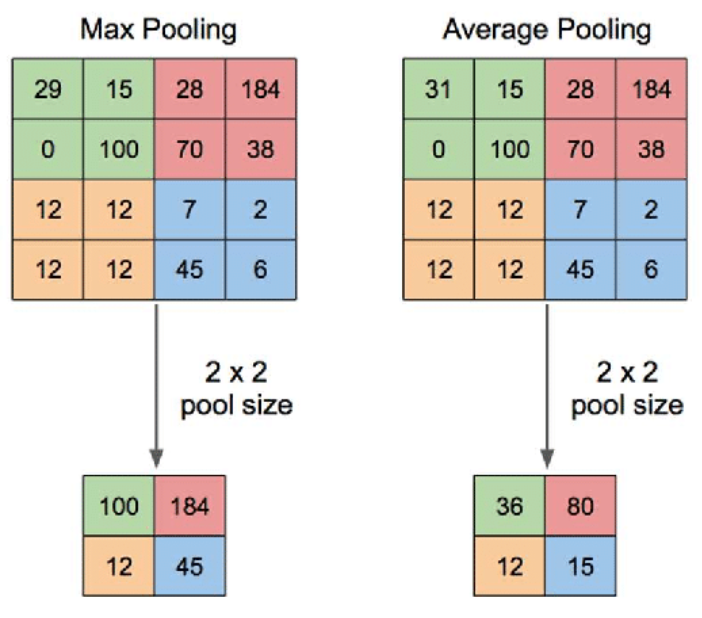
\includegraphics[width=400pt,height=250pt]{pictures/pooling.PNG}
  \caption{Max pooling operation on the left and average pooling operation on the right.\cite{pooling}}
  \label{fig:pooling}
\end{figure} 

The third step of a \ac{CNN} is to use the pooling layer. The main purpose of this operation is to make the detection of the features robust to the exact location of the eye (i.e. invariant to small translations). The different types of pooling operations are - max pooling and average pooling. It also helps in reducing the dimensionality of the input without losing too much information. This is done to make the computations faster down the deeper layers of the network. If the pooling operations are performed after every k pixels, then the next layer processes inputs that are k times lesser as shown in Fig. \ref{fig:pooling}. As the name suggest, the maximum value within the kernel is taken during max-pooling and the average value during average pooling. Since the number of parameters in a layer are dependent on the size of the input to the layer, it significantly reduces the computational overhead on using pooling operations.

\paragraph{Batch Normalization}
Another very important aspect in \ac{CNN} is batch normalization. In this step, it takes the output of the convolution layer and reassigns the pictures in the feature maps to a new mean and standard deviation. At first, the pixels values are normalized by calculating the z-score of all the pixels. It is then multiplied by a learnable parameter commonly referred as alpha which denotes the range and is then added to another learnable parameter beta which controls the offset value as shown in Eq. \ref{eq:batch_norm}. 
\begin{equation}
  \label{eq:batch_norm}
  x'= (\frac{(x-mean)}{standard \, deviation} \times alpha) + beta,
\end{equation}
where $x'$ is the normalized value after each batch, $x$ is the value of the pixel in the feature map. Batch normalization method is crucial because it handles the exploring gradient problem. 

\subsubsection{Autoencoders}
\begin{figure}
  \centering
  \begin{minipage}[t]{.45\textwidth}
    \centering
    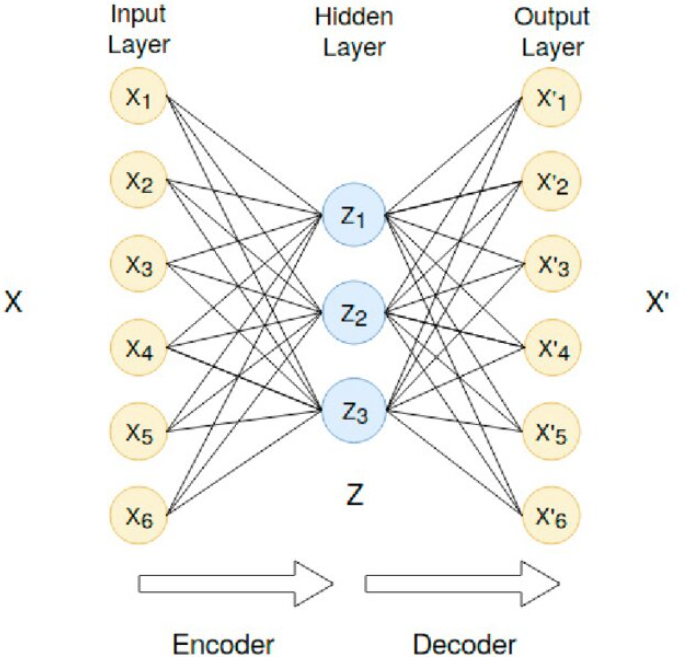
\includegraphics[width=200pt,height=150pt]{pictures/undercomplete_autoencoder.png}
    \captionof{figure}{Architecture of an undercomplete autoencoder.\cite{undercompleteautoencoder}}
    \label{fig:undercompleteautoencoder}
  \end{minipage}%
  \hspace{1cm}
  \begin{minipage}[t]{.45\textwidth}
    \centering
    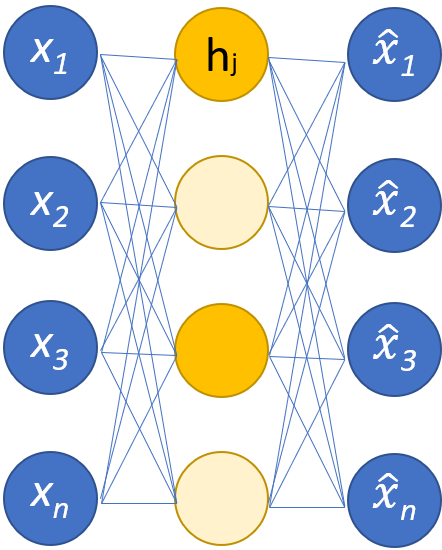
\includegraphics[width=200pt,height=150pt]{pictures/sparse_autoencoder.png}
    \captionof{figure}{Architecture of a single layer sparse encoder. The hidden nodes in bright yellow are active, while the ones in light yellow are set to zero, hence inactive\cite{autoencoder}}
    \label{fig:sparse_autoencoder}
  \end{minipage}
\end{figure}
Autoencoders are a special type of feedforward neural network in which the output tries to reconstruct the input. It is predominantly used in unsupervised learning for the tasks if dimensionality reduction, learning feature representations and for data compression. It tries the encode the input data into a more compact representation with lower dimensions called the "code"\cite{Goodfellow-et-al-2016} or "latent space". The idea is that this latent space representation should capture the most vital aspects of the input data. This is done by the first part of the network called the encoder. The second part of the network, the decoder then tries to decode this compressed representation of the input data to reconstruct the original input data as accurately as possible. During the training of an autoencoder, the goal is to minimize this reconstruction loss, i.e. the difference between the original input data and the output of the decoder. There are different types of autoencoders - undercomplete autoencoders, convolutional autoencoders, regularized autoencoders and variational autoencoders.

\vspace{5mm}


Undercomplete autoencoders ensure that the dimension of the latent space representation is less than the dimension of the original input data as show in Fig.\ref{fig:undercompleteautoencoder}. The output of the decoder to be the exact copy of the input is of no use. Rather, if the dimension of the code is less than that of the input, then it ensures that the autoencoder learns those representative features of the input data which are most salient\cite{Goodfellow-et-al-2016}. Convolutional autoencoders are an extension of traditional autoencoders where convolution layers are used as building blocks in both the encoder and the decoder part of the autoencoder. After training the network, the encoder part is used for extracting the features of the data and the decoder part is used for the reconstruction of the input data.

\vspace{5mm}

\begin{figure}[t]
  \centering
  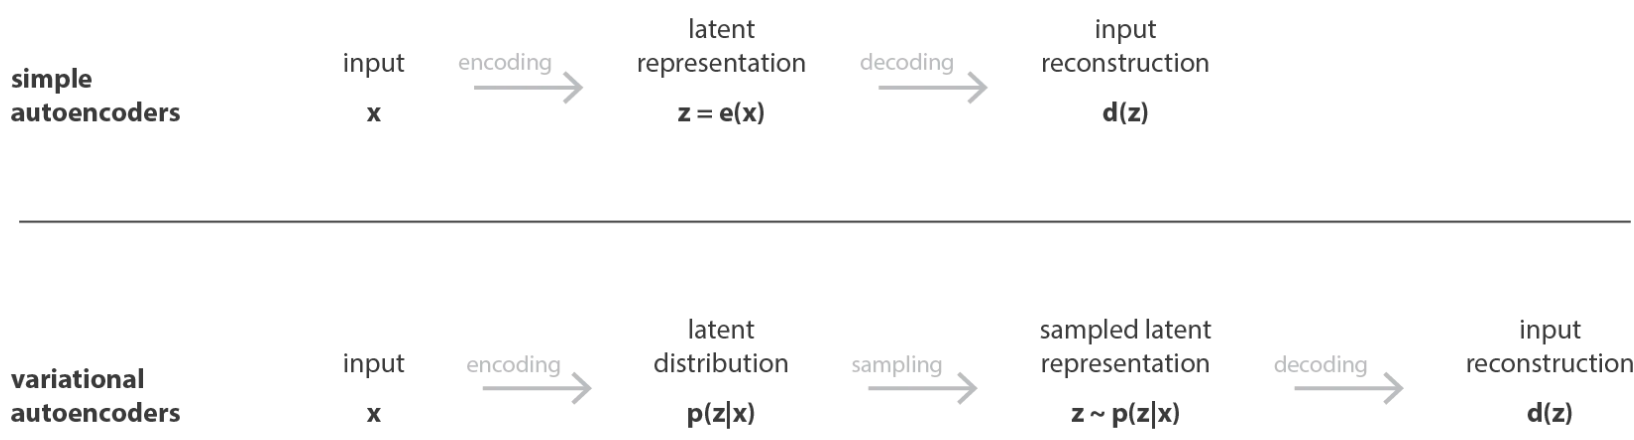
\includegraphics[width=400pt,height=150pt]{pictures/vae.png}
  \caption{Difference between a vanilla autoencoder and a \ac{VAE}.\cite{vae_image}}
  \label{fig:vae}
\end{figure} 
Regularized autoencoders are a special type of autoencoders that employs one or more regularization techniques to prevent the model from overfitting. The different types of regularizations used are L1 or L2 Regularization which add a penalty to the loss function depending on L1 or L2 norm of the model weights. As a result of this, the model is capable of learning sparse representation of the training data where many weights are set to a very small value or zero as shown in Fig\ref{fig:sparse_autoencoder}. Dropout is also used as a regularization technique where a percentage of the model's nodes are set to zero during training so that the model doesn't rely heavily on the weight of any particular node, thus, preventing overfitting and improving generalization on unseen data. 

\vspace{5mm}

The previously mentioned regularization techniques give rise to a variation of regularized autoencoders called the sparse autoencoders\cite{ng2011sparse}. Sometimes noise is also added to the training data or the hidden layers of the model to increase the robustness the model giving rise to denoizing autoencoders\cite{vincent2008extracting}. One more regularization technique is to apply a contractive regularization term based on Frobenius norm of the Jacobian matrix of the model's hidden layer activations with respect to the input data\cite{rifai2011contractive,autoencoder}. This ensures that a small neighborhood of the input data corresponds to a small neighborhood in the latent space representation, which means small perturbations in the input data leads to small or zero variation in the latent space representation\cite{rifai2011contractive,autoencoder}. By doing so, it makes the model more robust to small changes in the input data, thus, preventing overfitting.

\vspace{5mm}

\ac{VAE}s are a distinct type of autoencoders which produces latent space representations that are continuous. This allows random sampling and interpolation for the generation of new datapoints. The difference between a vanilla autoencoder and a \ac*{VAE} is shown in Fig.\ref{fig:vae}. Instead of producing a single vector for the latent space representation, it generates two vectors: a vector of means $\mu$ and a vector of standard deviations $\gamma$ for all datapoints. An encoding is then sampled from a distribution with mean $\mu$ and standard deviation $\gamma$. Thus, even for the same input, i.e. when the mean and the standard deviation are the same, the sampled encoding would vary because of the involvement of the sampling procedure. The mean vector controls the position where the encoding of the input should have its centre and the standard deviation controls the area over which the sampled encoding is allowed to vary from the mean. As a result of this, the decoder learns to decode not just the encoding of a single point but also the points in the neighborhood and hence a continuous latent space representation is obtained. In order to ensure that the latent space representation satisfies that the nearby encoding are similar to each other on a local scale while also facilitating interpolation on a global scale \ac{VAE}s jointly optimizes the reconstruction loss and the \ac*{KL}\cite{kullback1951information} loss.\cite{kingma2019introduction,vae}

\subsubsection{Siamese Network}
\begin{figure}
  \centering
  \begin{minipage}[t]{.45\textwidth}
    \centering
    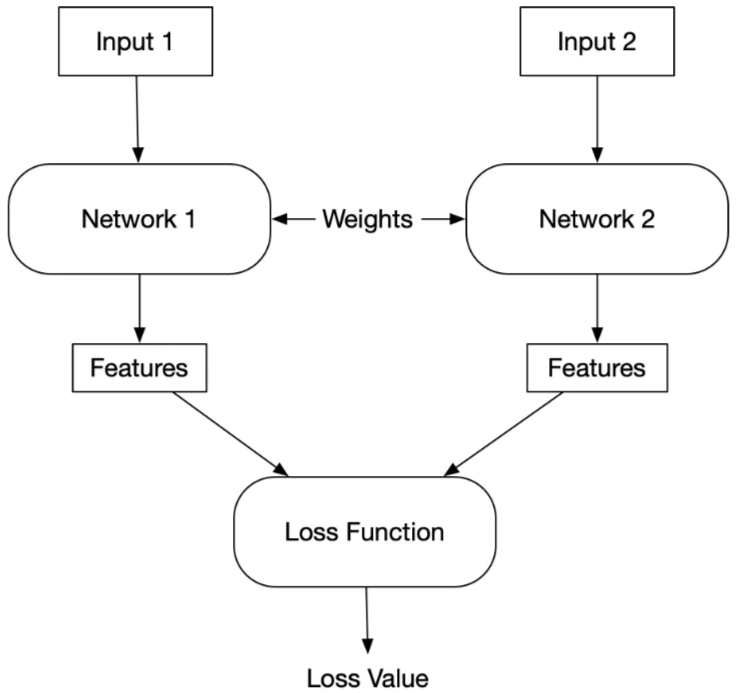
\includegraphics[width=200pt,height=120pt]{pictures/siamese_network.png}
    \captionof{figure}{A generic Siamese Network.\cite{siamese_network}}
    \label{fig:siamese_network}
  \end{minipage}%
  \hspace{1cm}
  \begin{minipage}[t]{.45\textwidth}
    \centering
    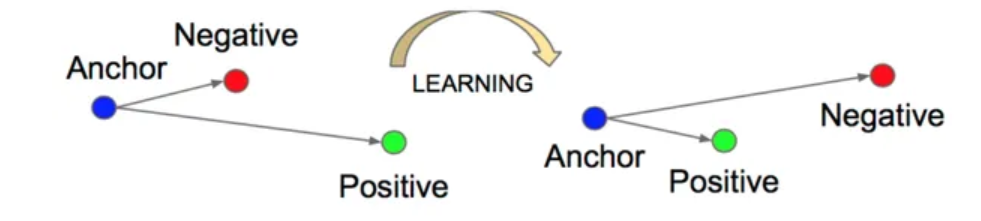
\includegraphics[width=200pt,height=100pt]{pictures/triplet_loss.PNG}
    \captionof{figure}{Before (left) and after (right) minimizing triplet loss function\cite{triplet_loss}}
    \label{fig:triplet_loss}
  \end{minipage}
\end{figure}
Traditional deep learning models have shown ground breaking results in a multitude of applications like image recognition and classification, web scraping, speech recognition and caption generation. But it has a limitation that the models tend to perform well if the training and testing data points are from the same distribution. If the model is to be made capable to predict datapoints belonging to an unknown class, it needs to be re-trained with an abundant number of training samples from that class and then predict it with unseen samples of that class. This technique can often be computationally expensive and can increase expotentially if the number of classes increases. Also generating a huge number of samples for a new class of objects can be tedious and quite challenging in multiple scenarios. The Siamese Network\cite{koch2015siamese,bromley1993signature} is one such way to mitigate the above mentioned problem. The idea behind Siamese Networks is that two identical copies of the neural network with shared weights process two distinct datapoints as shown in Fig.\ref{fig:siamese_network}. Because the networks have shared parameters, it ensures that two very similar datapoints cannot have two different locations in the feature maps as both the networks evaluate the same function. In Siamese Networks, the model learns a similarity function, the loss function, which plays the pivotal role in determining how similar or dissimilar the datapoints are to one another. The two main loss functions used in Siamese Networks are contrastive loss function\cite{bromley1993signature} and triplet loss function\cite{balntas2016learning}. Since the goal of a Siamese Network is not to perform classification task on datapoints, rather to compute the similarity between them, contrative loss functions are more suited for this task as compared to cross-entropy loss functions, as it is for classification tasks.\cite{koch2015siamese}

\vspace{5mm}

\textbf{Contrastive loss} function evaluates how capable a Siamese Network is in deciding the similarity between two given datapoints as is given by Eq. \ref{eq:contrastive_loss}\cite{siamese_network, koch2015siamese}

\begin{equation}
  \label{eq:contrastive_loss}
  \mathcal{L}_{\textrm{con}}(Y,D_{w})= (1-Y)\frac{1}{2}(D_{w})^2 + (Y)\frac{1}{2}{max(0,m-D_{w})}^2,
\end{equation}
where $\mathcal{L}_{\textrm{con}}$ is the calculated contrastive loss, $D_{w}$ is the Euclidean distance between the outputs of the twin networks\cite{siamese_network}. Y takes the value 0 or 1. If the two datapoints belong to the same class then Y takes the value 0, otherwise it takes the value 1\cite{siamese_network}. max() is a function to choose the higher of the two values, 0 or $m-D_{w}$ where $m$ is the margin and has a value greater than 0\cite{siamese_network}. The usage of a margin in this equation ensures that the pair of datapoints which the dissimilar beyond this margin value are excluded while calculating the loss function\cite{siamese_network}. The euclidean distance between the embeddings of the two datapoints are given by the Eq. \ref{eq:euclidean_dist}.\cite{siamese_network, koch2015siamese}
\begin{equation}
  \label{eq:euclidean_dist}
  D_{w}(X_{1},X_{2})= \sqrt[2]{\{G_{w}(X_{1}) - G_{w}(X_{2})\}^2},
\end{equation}
where $G_{w}(X_{i})$ is the output of the twin network such that $i \in \{1,2\}$ as show in Fig.\ref{fig:siamese_network}.
\begin{figure}
  \centering
  \begin{minipage}[t]{.45\textwidth}
    \centering
    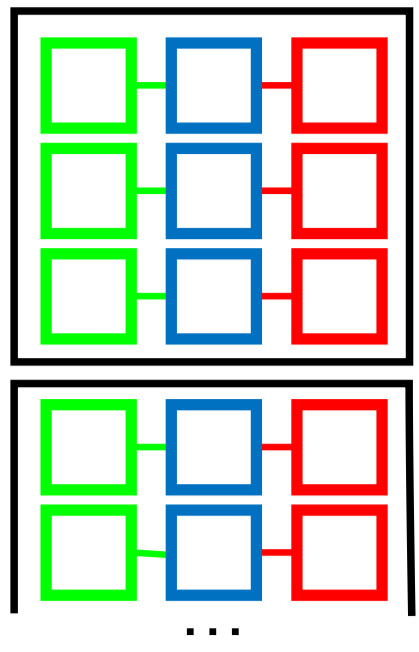
\includegraphics[width=100pt,height=120pt]{pictures/offline_triplet.jpg}
    \captionof{figure}{Minibatches in offline triplet mining. The green boxes are positive datapoints, the blue boxes are anchor datapoints and the red boxes are negative datapoints.\cite{siamese_leibe}}
    \label{fig:offline_triplet}
  \end{minipage}%
  \hspace{1cm}
  \begin{minipage}[t]{.45\textwidth}
    \centering
    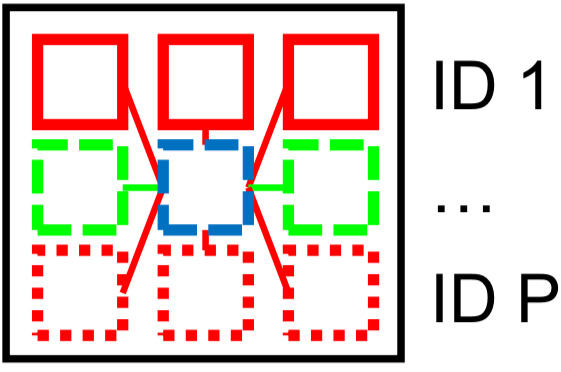
\includegraphics[width=100pt,height=120pt]{pictures/online_triplet.jpg}
    \captionof{figure}{Triplets constructed only within the minibatch. There are P object classes in the minibatch. The green boxes are positive datapoints, the blue boxe is the anchor datapoint and the red boxes are negative datapoints.\cite{siamese_leibe}}
    \label{fig:online_triplet}
  \end{minipage}
\end{figure}

\vspace{5mm}

\textbf{Triplet loss} function\cite{weinberger2009distance} trains the Siamese Network in a way that a triplet of datapoints are presented to the Siamese Network. By applying triplet loss the model tries to group the datapoints similar to the anchor datapoint, close to one another while increasing the distance between the anchor datapoint and the datapoints dissimilar to it as shown in Fig.\ref{fig:triplet_loss}. In order to do so, a positive value called margin is used which increases the distance between dissimilar datapoints and also eliminates the output of any trivial solution. Euclidean distance or cosine distance is used as the distance metric while calculating the triplet loss and shown in Eq. \ref{eq:triplet_loss}. \cite{hermans2017defense,siamese_network}
\begin{equation}
  \label{eq:triplet_loss}
  \mathcal{L}_{\textrm{tri}}(a,p,n)=\sum_{\substack{a,p,n \\ y_{a}=y_{p}!=y_{n}}} max(0,d(a,p)-d(a,n)+margin),
\end{equation}
where $y_{x}$ is the class label for the datapoint $x$ for $x \in \{a,p,n\}$, $a$ is the anchor datapoint, $p$ is the positive example having the same class label as the anchor datapoint and $n$ is the negative example having a different class label as compared to the anchor datapoint. But there are some practical problems related to the use of triplet loss function. The number of possible triplets grow cubically with the increase in the size of the dataset. Also most of the triplets are often uninformative. Thus, mining "hard triplets" or the ones crucial for the learning of the model becomes a challenging task. As per the definition of the triplet loss function, the triplets can be of three types: easy triplets, hard triplets and medium hard triplets. The triplets which satisfy the condition $d(a,p)+margin<d(a,n)$ results to the loss value being 0, hence are called the easy triplets\cite{triplet_loss}. For the triplet for which the negative datapoint is closer to the anchor as compared to the positive datapoint i.e. $d(a,n)<d(a,p)$ are the examples of hard triplets.\cite{triplet_loss} And the medium hard triplets are the ones where the negative datapoints are not closer to the anchor datapoint as compared to the positive datapoint but still results in positive loss i.e. $d(a,p)<d(a,n)<d(a,p)+margin$.\cite{triplet_loss} Thus, the medium hard triplets are the most essential for the model training as they constitute for the most useful information. Two triplet mining procedures are used to mitigate the issue of excessive computational overhead with increase in dataset size. They are offline triplet mining and online triplet mining. In offline hard triplet mining, at first the dataset is manually processed to find hard triplets and then they are used for training the model. But manually finding the hard triplets can be quite tedious. Online triplet mining is a better approach as compared to the one mentioned above. The model is trained in minibatches of the dataset as shown in Fig.\ref{fig:offline_triplet}. Using only the triplets that were mined from the dataset could be a wasteful design choice in such scenario. So in a minibatch, it contains way more potential triplets than the ones that were mined. So each member of another triplet becomes an additional negative datapoint example. But both hard positive and hard negative datapoints are required for training. An even better design to mitigate that would be to choose let's say $c$ datapoints from P different classes in the dataset, where the $k$ positive examples serve as hard positives while the rest of the datapoints in the minibatch serve as hard negatives as shown in Fig.\ref{fig:online_triplet}.\cite{hermans2017defense}

\vspace{5mm}

Thus, Siamese Networks are very robust to the class imbalance in dataset which is very common in real datasets. Since it depends on very few datapoints of a particular object class, it has good generalization capabilities for unseen datapoints in the future. They are also very robust to small perturbations in the datapoints due to difference in lighting conditions orientation or background, as they keep similar objects close to each other even if the datapoints are slightly different. Since the Siamese Networks places similar datapoints together while increasing the distance between dissimilar datapoints, they are often useful for learning semantic similarity within the datapoints. However despite its benefit, training a Siamese Network takes longer as compared to traditional neural networks because it involves learning from quadratic pair of datapoints.\cite{siamese_network, koch2015siamese}

\subsection{Clustering Algorithms}
\label{sec:Clustering_Algorithms}
\begin{figure}[t]
  \centering
  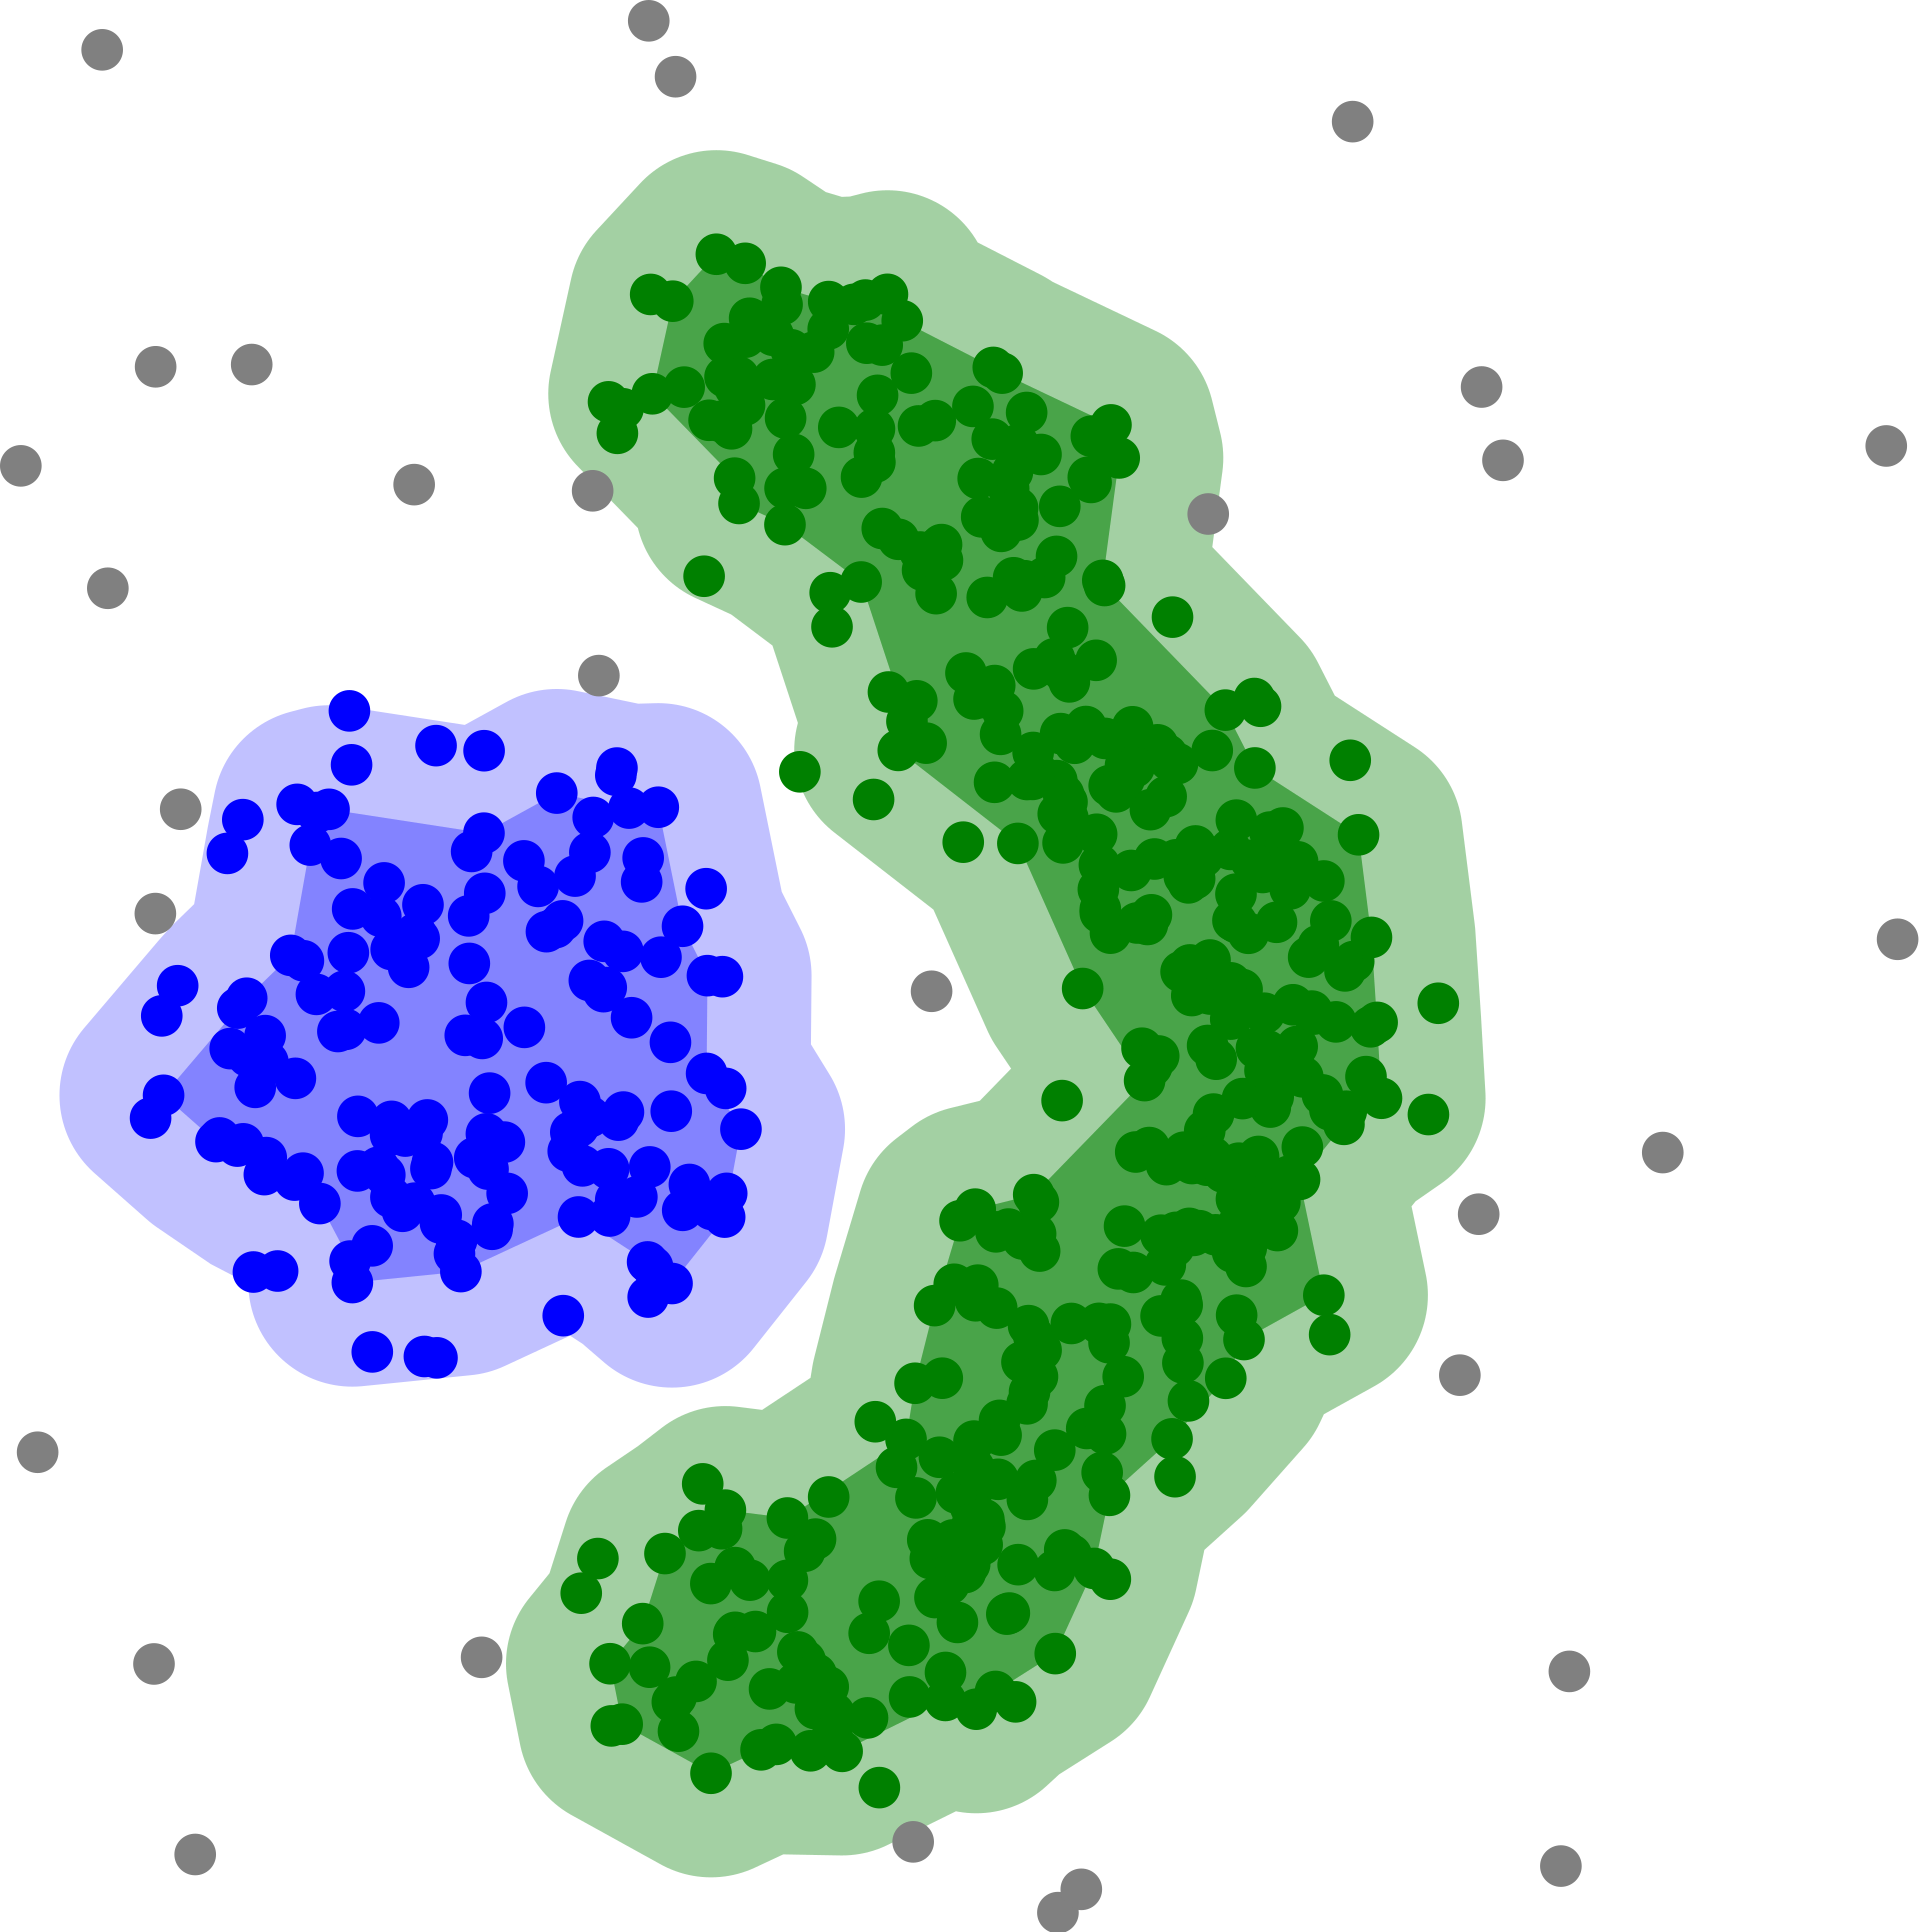
\includegraphics[width=200pt,height=150pt]{pictures/DBSCAN-density-data.png}
  \caption{\ac{DBSCAN} can find non-linearly separable non-convex clusters.\cite{dbscanWiki}}
  \label{fig:dbscan}
\end{figure} 
When the dataset does not have any labelled data, then it is said to be unsupervised learning. In this case, there is no ground truth available to measure the correctness of the outputs generated by the \ac{ML} models. The primary focus of unsupervised learning is to find hidden and interesting pattern in the data. Unsupervised learning is of utmost importance in the \ac{AI} world as several real world datasets do not have available annotations, which requires a lot of human effort. Unsupervised learning algorithms can be broadly categorized into the following: domains-clustering, dimensionality reduction and association analysis. Clustering algorithms aim at grouping unlabelled data into groups or clusters based on how similar or dissimilar the datapoints are to one another. It can reveal underlying hidden pattern in the data and is used in applications like image segmentation, fraud detection, etc. 

\vspace{5mm}

Dimensionality reduction reduces the number of irrelavant features or dimensions of the dataset. The inclusion of more features does help in the better representation of the dataset but it also significantly increases the memory consumption and complexity to work with it. Also it is often difficult to visualize real-life datasets with too many features. Association analysis is a rule-based unsupervised learning method that reveals the relationship between attributes in the dataset. It is used in applications like market analysis, intrusion detection, etc. Clustering algorithms can be broadly classified into the following categories: density-based, distribution-based, graph-theory based and hierarchical-based.\\
\begin{figure}
  \centering
  \begin{minipage}[t]{.45\textwidth}
    \centering
    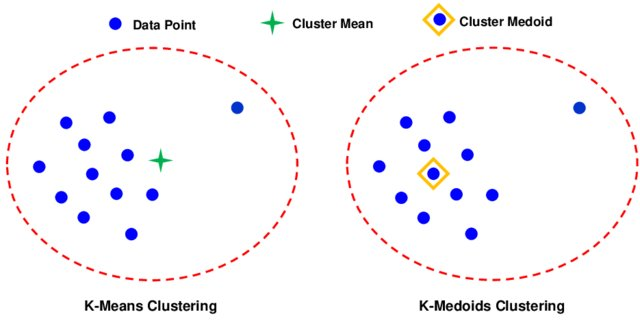
\includegraphics[width=200pt,height=150pt]{pictures/The-graphical-representation-of-the-difference-between-the-k-means-and-k-medoids_W640.jpg}
    \captionof{figure}{Difference between k-means and k-medoids.\cite{kmean-kmedoid}}
    \label{fig:kmean-kmedoid}
  \end{minipage}%
  \hspace{1cm}
  \begin{minipage}[t]{.45\textwidth}
    \centering
    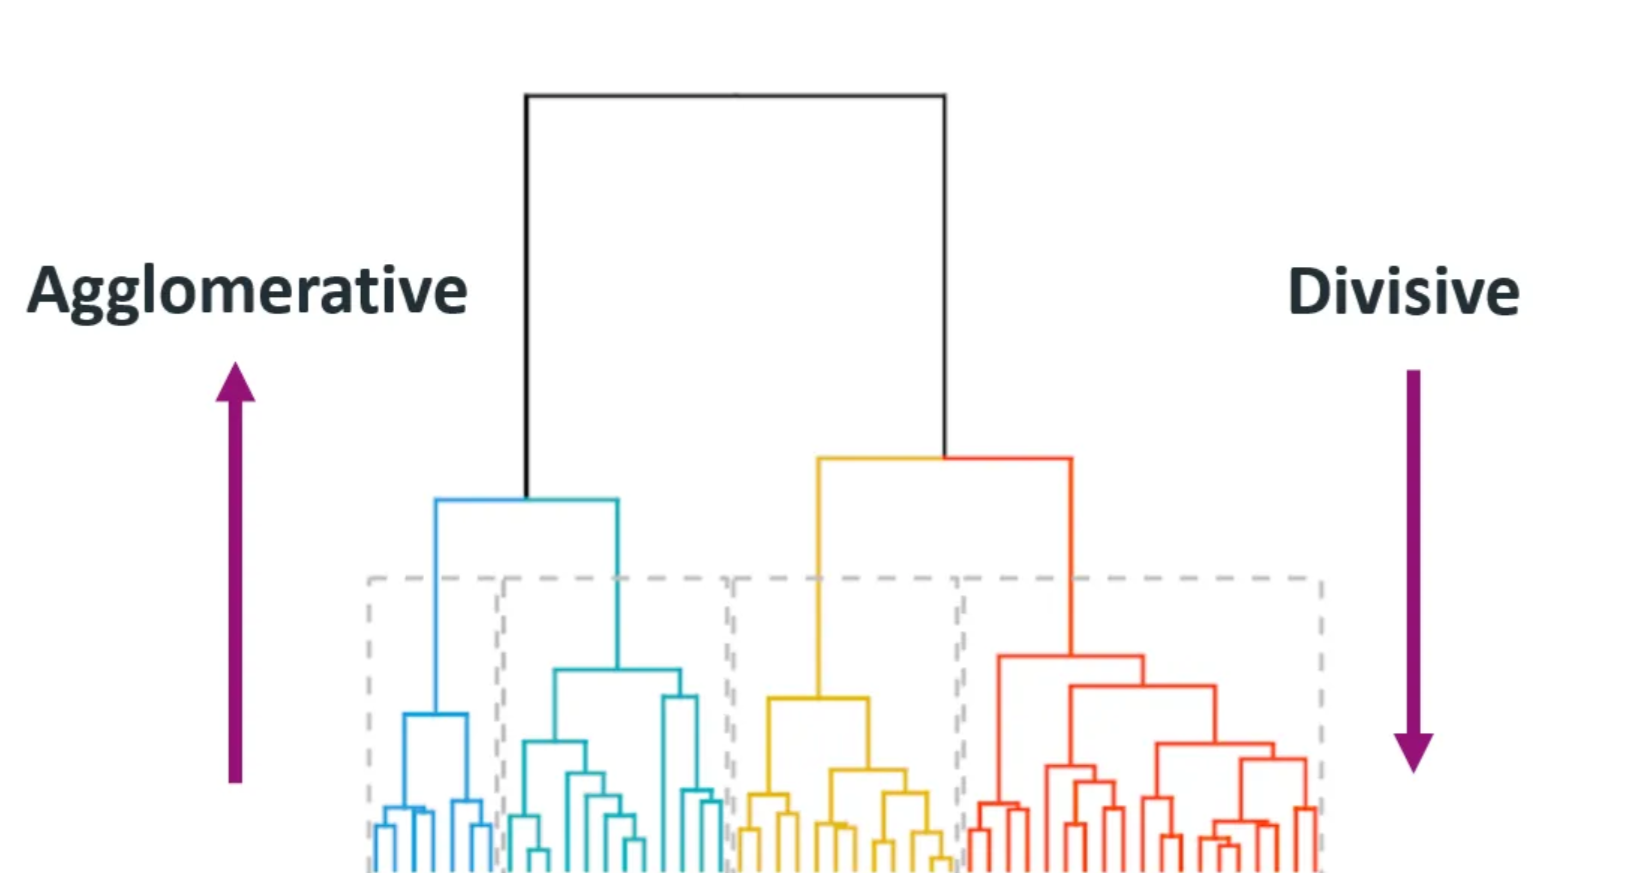
\includegraphics[width=200pt,height=150pt]{pictures/dendogram.png}
    \captionof{figure}{A dendogram in hierarchical clustering.\cite{dendogram}}
    \label{fig:dendogram}
  \end{minipage}
\end{figure}
\subsubsection{Density-Based Clustering}
 In density-based clustering, the algorithm looks for areas of high concentration of the datapoints and groups them as a cluster. The benefit of this algorithm is that the shape of a cluster is not limited and hence doesn't necessarily have to be convex in nature as show in Fig. \ref{fig:dbscan}.
Moreover, these algorithms are also very robust to outliers as they do not force the outliers to belong to any category but are rather ignored as it is unlikely that outliers can form an area of high concentration of datapoints. The experiments on this thesis have been carried on two such density-based clustering algorithms called \ac{DBSCAN}\cite{dbscan} and \ac{HDBSCAN} algorithms\cite{hdbscan}. The available scikit-learn python library implementations were used for this purpose\cite{scikit-learn}. The \ac{DBSCAN}\cite{dbscan} algorithm  does not require the users to define the number of clusters to be generated which doesn't force dissimilar datapoints to belong to the same cluster. However, this algorithm was still sensitive to two parameters $\epsilon$, the maximum distance between the datapoints to be considered in the same cluster and the minimum number of samples in the cluster which the user needs to define \cite{scikit-learn}. But finding an optimum value for these parameters often require domain expertise and are dependent on the data. The \ac{HDBSCAN}\cite{hdbscan} algorithm mitigates this issue and thus, does not require the user to define these two parameters. It is a hierarchical density-based clustering that performs the \ac{DBSCAN} algorithm over multiple $\epsilon$ values to find the most stable result. 

\subsubsection{Distribution-Based Clustering}
\label{sec:Distribution_based_Clustering}
In distribution-based algorithms, a datapoint is said to be a member of the cluster depending on the probability of its membership to the cluster. The more the distance of a point increases from the centre of the cluster, the less is its probability of belonging to that cluster. Centroid-based algorithms groups the datapoints based on some initial cluster centres. Once all the datapoints are softly assigned to some cluster membership, the cluster centres are recalculated and this process is iterated until convergence. These algorithms are sensitive to the initial parameters like the cluster centres chosen in the first step. Another major disadvantage of these clustering algorithms are that they always form spherical clusters. The user also needs to define the number of clusters the dataset is to be grouped in, which makes it sensitive to outliers. However, these algorithms can be executed very fast and two such algorithms were used during the experiments in this thesis- k-means\cite{kmeans}and k-medoids\cite{kmedoids}. In k-means, the mean of the datapoints of the clusters is assigned as the cluster-centroid. It might not be an actual datapoint in the dataset, rather a blurred, noisy average of a datapoints in the cluster. On the contrary, the k-medoids algorithm assigns an actual datapoint of the dataset, that is most centrally located as the cluster centroid as shown in Fig.\ref{fig:kmean-kmedoid}. Thus, k-medoids is more robust to outliers and noises as compared to k-means.\cite{arora2016analysis}

\subsubsection{Hierarchical-Based Clustering}
Hierarchical-based clustering algorithms form a hierarchy of clusters. Datapoints in a cluster are more similar to each other as compared to other groups. This hierarchy of clusters is visualized by a hierarchy tree called dendograms. Hierarchical clustering algorithms can be of two types - agglomerative and divisive. In agglomerative clustering, each datapoint is considered as a separate cluster in the first step. Then these clusters are merged into one another until only one cluster remains. Thus, at the end, the last level cluster consists of all the datapoints in the dataset. The divisive method is the reverse procedure of the agglomerative method. In the beginning, all the datapoints are considered to be in a single cluster and gradually the cluster is broken into smaller clusters, until each cluster consists of only one datapoint. A visual representation of a dendogram has been shown in Fig.\ref{fig:dendogram}.\cite{murtagh2012algorithms}

\subsubsection{Graph Theory-Based Clustering}
Spectral clustering is a powerful machine learning tool which divides datapoints into meaningful groups based on their similarity. The concept of spectral clustering has its root in the graph theory. It tries to determine the node communities in a graph by looking at the edges that connect them. It is specially useful when the dataset cannot be linearly-separated. The affinity matrix of the datapoints, which gauges the pairwise similarity between points, is the basis for spectral clustering. It works by creating a graph representation of the data, in which datapoints are represented by nodes and the degree of similarity between the points indicated by edges. After that the eigenvectors of a matrix is obtained from this graph which is used to create the embeddings of the datapoints in a lower dimensional space.  The embedded points are then divided into clusters by using a common clustering algorithm, usually the distributed based clustering algorithm k-means, where each entry in the embedding matrix is the representation of the datapoints in the lower dimensional space. Spectral clustering has shown promising results with datasts that have complex structures and non-linear separability, which makes it a useful tool in varity of fields, such as social network analysis, image segmentation and dimensionality reduction\cite{von2007tutorial}. A comparison between the results of k-means and spectral clustering in the presence of non-globular clusters in shown in Fig. \ref{fig:spectral}.\cite{demmel1999cs}
\begin{figure}[t]
  \centering
  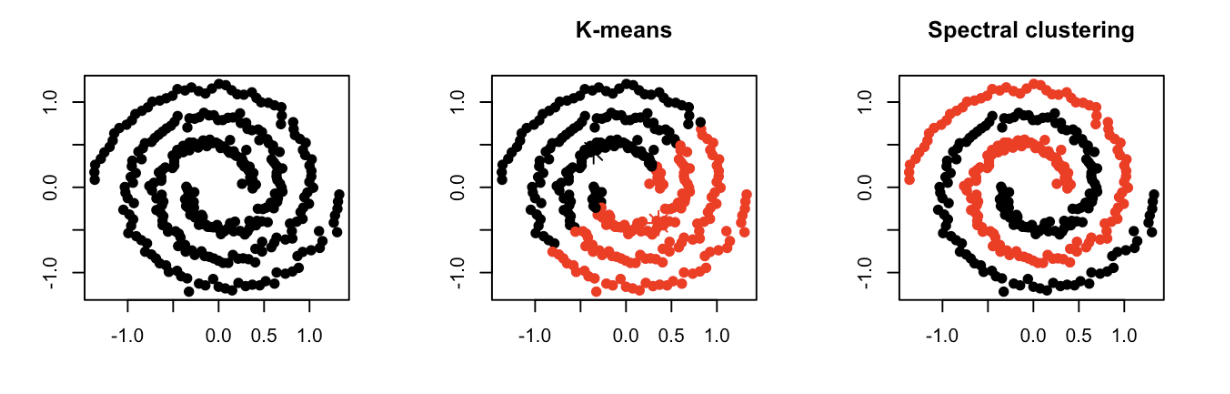
\includegraphics[width=400pt,height=200pt]{pictures/spectral.PNG}
  \caption{A comparison between the results of k-means clustering and spectral clustering. The image in the left shows the points that need to be clustered.\cite{palmer2021spectral}}
  \label{fig:spectral}
\end{figure} 

\subsection{Evaluation Metrics for Clustering Algorithms}
The ground truth or labels are available in supervised learning. So to determine the quality of the clustering algorithm the level of accuracy is calculated by comparing the labels predicted by a model to the ground truth. But most real world datasets do not have a ground truth. Therefore, it makes it challenging in unsupervised learning paradigm to determine the quality of the clustering algorithm. A good clustering algorithm is still expected to have little difference between the objects in a cluster i.e. small within-cluster variance and more difference between objects from different clusters i.e. large between-cluster variance. Thus, the evaluation metrics used in the literature could be categorized into two broad groups: extrinsic measures and intrinsic measures, depending on the availability of the ground truth. Extrinsic measures, when the ground truth is available uses metrices like Rand Index, Mutual Information, V-measure and Fowlkes-Mallows Scores. Intrinsic measures, when the ground truth is not available mostly uses Silhouette Score, Calinski Harabaz index and David Bouldin index.

\subsubsection{Silhouette Score}
Silhouette Score is used to calculate the distance between points within a cluster as compared to its distance from the points in the neighbouring cluster and is given by Eq. \ref{eq:silhouette_score}.
\begin{equation}
  \label{eq:silhouette_score}
  \mathit{S_{c}}= \mathit{\frac{(n_{c}-i_{c})}{max(n_{c},i_{c})}},
\end{equation}
where $S_{c}$ is the Silhouette Coefficient, $n_{c}$ is the average of the nearest-cluster distance of each datapoint and $i_{c}$ is the average distance between the datapoint within the cluster. The Silhouette coefficient lies within the range $[-1,1]$, where the the more closer the coefficient is to 1, the better is the clustering results. When the Silhouette Coefficient is close to 0, it implies that the datapoints are on or very close to the decision boundary between adjacent clusters, whereas negative values imply that the datapoints have been wrongly classified. But the drawbacks of using this metric is, that is tends to favour dense and convex clusters. Since it takes into account the average of the distance within a cluster as well as between adjacent clusters, it doesn't perform well if different clusters have a significant difference in their respective sizes, which is quite a common phenomenon in real world datasets. The chosen distance metric for the calculation of the Silhouette score also has a significant effect on it and can lead to very different results.

\subsubsection{Calinski-Harabasz Index}

Calinski-Harabasz Index(C-H Index) or the Variance Ratio Criterion is used to measure the dispersion between the datapoints within a cluster as compared to in-between clusters as in given by Eq. \ref{eq:c-h index}.
\begin{equation}
  \label{eq:c-h index}
  \mathit{S_{CH}}= \mathit{\frac{tr(B_{k})}{tr(W_{k})}} \times \mathit{\frac{(n_{E}-k)}{k-1}},
\end{equation}
where $S_{CH}$ is the C-H Index, $tr(B_{k})$ is the trace of the in-between cluster dispersion matrix. $B_{k}$ is in Eq. \ref{eq:Bk}  and $tr(W_{k})$ is the trace of the within-cluster dispersion matrix. $W_{k}$ is shown in Eq. \ref{eq:Wk}.
\begin{equation}
  \label{eq:Bk}
  \mathit{B_{k}}= \mathit{\sum_{q=1}^{k}n_{q}(c_{q}-c_{o})(c_{q}-c_{o})^T}, 
\end{equation}
\begin{equation}
  \label{eq:Wk}
  \mathit{W_{k}}= \mathit{\sum_{q=1}^{k}\sum_{x \in C_{q}}(x-c_{q})(x-c_{q})^T}, 
\end{equation}
where, $C_q$ is the collection of points in cluster $q$, $c_{q}$ is the centroid of the cluster $q$ and $c_{o}$ is the overall centroid of the datapoints. $B_{k}$ calculates the quality of the separation between two clusters, i.e. higher the value of $B_{k}$, better it is. $W_{k}$ calculates the distance of a datapoint ($x$) from the centroid of the cluster and thus, measures the cohesiveness or compactness of the datapoints within a cluster, i.e smaller the value of $W_{k}$ the better it is. Distribution-based clustering algorithms like k-means tries to minimize the value of $W_{k}$. Thus, according to the equation of C-H Index in Eq. \ref{eq:c-h index}, the higher the C-H index, the better is the clustering results. Because sum-of squared Euclidean distance is used to calculate the distance of the datapoints from their respective cluster centroids, C-H Index tends to favour convex clusters, which is a major drawback of using this metric similar to that in Silhouette Coefficient.\cite{chindex}

\subsubsection{David-Bouldin Index}

David-Bouldin Index is another metric used for evaluating clustering algorithms, which uses only the intrinsic features of the dataset and doesn't require any ground truth labels. David and Bouldin proposed R,a measure to calculate cluster similarity that satisfied the following conditions\cite{vergani2018soft}:
\begin{itemize}
  \item $R(S_i, S_j, M_{ij}) \geq 0$
  \item $R(S_i, S_j, M_{ij}) = R(Sj, S_i, M_{ij})$
  \item $R(S_i, S_j, M_{ij}) = 0$ iff $S_i = S_j$
  \item if $S_i = S_j$ and $M_{ij} < M_{ik}$, then $R(S_i, S_j,M_{ij}) > R(S_i, S_k,M_{ik})$  
  \item if $Mij = M_{ik}$ and $Sj > Si$, then $R(Si, Sj, M_{ij}) > R(Si, Sk, M_{ik})$
\end{itemize}
where $M_{ij}$ is the distance between the centroids of the clusters $i$ and $j$ and $S_i$ and $S_j$ are their respective dispersion measures. The conditions enforce that the cluster similarity measure R is non-negative and symmetrical in nature. It becomes 0 if and only if the dispersions of the two clusters disappear. If the distance $M_{ij}$ increases even if $S_i$, $S_j$ are constant, then the cluster similarity measure R decreases and vice versa. Also if $M_{ij}$ remains constant and $S_i$, $S_j$ increases, then R increases. Thus, the David-Bouldin Index was defined as the average of the similarities of each cluster as in Eq. \ref{eq:dbi}, using the same notations as the authors.
\begin{equation}
  \label{eq:dbi}
  \mathit{\bar{R}}= \mathit{\frac{1}{C}\sum_{i=1}^{C}R_i}, 
\end{equation}
where C is the total number of clusters and $R_i$ is the $max_{j \neq i}{R_{i,j}}$. Thus, $\bar{R}$ or the David-Bouldin Index is the average of the similarity measures R of each cluster with its most similar cluster. Thus, David-Bouldin Index has a lower bound of 0, while a higher value means bad clustering. In other words, the less is the average similarity, the better is the clustering results. Because of this, it acts as a good measure to decide on the number of clusters that actually exists in the dataset. Therefore, this index can be used to determine the number of clusters in distribution-based clustering algorithms like k-means. $R_{i,j}$ is more formally defined as in Eq. \ref{eq:ri}.
\begin{equation}
  \label{eq:ri}
  \mathit{R_{i,j}}= \mathit{\frac{S_i + S_j}{M_{ij}}}. 
\end{equation}
The dispersion measure of a cluster $i$ is defined by $S_I$ as in Eq. \ref{eq:si}.
\begin{equation}
  \label{eq:si}
  \mathit{S_i}= \mathit{\left\{\frac{1}{N_i}\sum_{j=1}^{N_i} \lVert X_j - A_i \rVert^q\right\}^{\frac{1}{q}}}, 
\end{equation}
where $N_i$ are the number of datapoints in the cluster $i$ and $X_j$ are the respective vector representations of the datapoints in the cluster $i$. For $q=1$, The dispersion measure $S_i$ is the average Euclidean distance of the vector representation of the datapoints from the centroid of the cluster $i$, while for $q=2$, it is the standard deviation of the metric about the datapoints in the cluster with respect to its centroid \cite{vergani2018soft}. It is different as compared to the distance defined between the centroids of the clusters which are defined as in Eq. \ref{eq:mij}.
\begin{equation}
  \label{eq:mij}
  \mathit{M_{i,j}}= \mathit{\left\{\sum_{k=1}^{N} \lVert a_{ki} - a_{kj}, \rVert^p\right\}^{\frac{1}{p}}} 
\end{equation}
where $a_{ki}$ is the k-th component of the vector representation of $a_i$ which is the centroid of the cluster $i$. $M_{i,j}$ is the Minkowski metric of the centroids of the clusters $i$ and $j$, i.e. when $p=1$, it is the Manhattan distance and when $p=2$ it is the euclidean distance between the centroids. When both p and q are 2, then $R_{i,j}$ is the Fisher similarity measure between the two clusters \cite{vergani2018soft}. But this metric too is not without its limitations. It is not robust to noise and outliers, thus, giving an incorrect sense of good clustering. This index too is biased towards spherical clusters with similar sizes, thereby making it inappropriate for many real world applications. Moreover, since it is a metric of the clustering results on a global level and gives no information about the individual clusters, even a single "too good" or "too bad" cluster can heavily influence the final result.

\subsection{Transfer Learning}
Transfer learning is an improvement in machine learning techniques where a model trained for a particular task. Let's say task 1 is different from another task, task 2. It uses the knowledge learnt by the model in the previous task to be adapted for the new task. Transfer learning has its benefits in a multitude of applications because real world problems doesn't necessarily always have an abundant amount of labelled data which can be used to train a model from scratch \cite{weiss2016survey}. It can be used for tasks which intend to solve different but related problems \cite{weiss2016survey}. In other words, if the domain of the data for task 2 is similar to that of task 1, transfer learning can be used as shown in Fig. \ref{fig:source_target}. Several approaches have been adapted to use transfer learning. Let's say one wants to solve task $T_{1}$ but don't have adequate data to train a deep neural network for it. But there is ample data to solve a similar task $T_{2}$. So one can train a model for task $T_{2}$ and then use it for task $T_{1}$. It might be needed to re-train only the later layers or all the layers of the model but that heavily depends on the problem at hand. Another approach that could be adapted is to use an existing pre-trained network. There are a lot of available open-source models which can be re-trained and re-used depending on the problem. Some of the popular models that are used as pre-trained models in transfer learning are Oxford VGG Model \cite{simonyan2014very},Google Inception model \cite{szegedy2015going} and Microsoft ResNet model \cite{he2016deep}. Another approach could be to use transfer learning for the purpose of feature extraction. Transfer learning has found a lot of application in the domain of computer vision and natural language processing because it requires a lot of data for training such complex models from scratch. In the domain of computer vision, it is known that the early layers of a deep neural network focuses on learning the low level features like the detection of edges, while the middle layers focus on learning the mid level features like the detection of shapes. In transfer learning, these pre-trained early and middle layers generally referred to as backbones could be used verbatim and only the latter layers which focus on the high level features could be re-trained for the new task as shown in fig \ref{fig:transfer_learning}.
\begin{figure}
  \centering
  \begin{minipage}[t]{.45\textwidth}
    \centering
    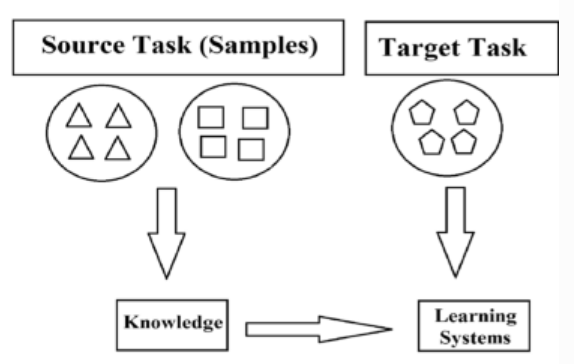
\includegraphics[width=100pt,height=120pt]{pictures/source_target.PNG}
    \captionof{figure}{Model trained for a task in the similar domain is re-used for a new task.\cite{hosna2022transfer}}
    \label{fig:source_target}
  \end{minipage}%
  \hspace{1cm}
  \begin{minipage}[t]{.45\textwidth}
    \centering
    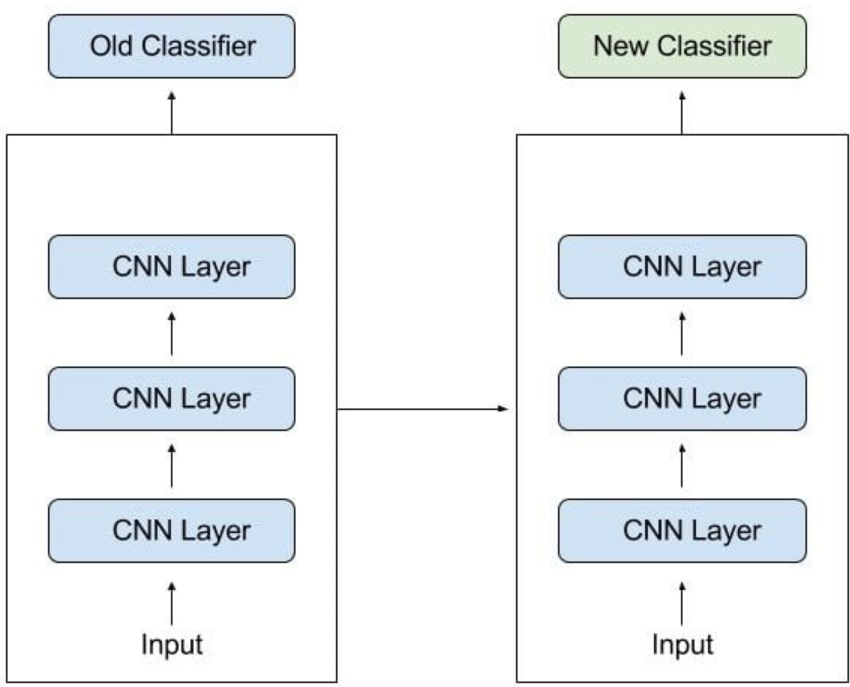
\includegraphics[width=100pt,height=120pt]{pictures/transfer_learning.PNG}
    \captionof{figure}{A model trained on a different task is adapted to be used for a new task.\cite{transfer_learning}}
    \label{fig:transfer_learning}
  \end{minipage}  
\end{figure}
Transfer learning has numerous advantages like significant reduction in the amount of training time\cite{liu2019exploring}, improvement in performance for some neural networks\cite{pan2011transfer} and less reliance on a huge amount of data\cite{duan2012learning,kulis2011you,zhu2011heterogeneous}.  
\subsubsection{Definition}
According to \cite{weiss2016survey,pan2009survey}, transfer learning can be formally defined as the following. A domain $\mathcal{D}$ of the input data, with the feature space $\mathcal{X}$ and a marginal probability distribution $P(X)$ such that $X=\{x_{1},.....,x_{n}\} \in \mathcal{X}$, where $n$ is the number of feature vectors in $X$. In the given input data domain $\mathcal{D}$, the task $\mathcal{T}$ has a label space $\mathcal{Y}$ and a predictive function $f(\cdot)$ which is learned from the feature vector and label pairs $(x_{i},y_{i})$ such that $x_{i} \in \mathcal{X}$ and $y_{i} \in \mathcal{Y}$ and $f(x)$ is the learner that predicts the label value for x. As per the above definition, the source domain is defined as $\mathcal{D_{\mathcal{S}}}$ and the corresponding source task as $\mathcal{T_{\mathcal{S}}}$.The target domain is defined as $\mathcal{D_{\mathcal{T}}}$ and the corresponding target task as $\mathcal{T_{\mathcal{T}}}$. Transfer learning aims at improving the target predictive function $f_{\mathcal{T}}(\cdot)$ by using the related information from $\mathcal{D_{\mathcal{S}}}$ and $\mathcal{T_{\mathcal{S}}}$ where $\mathcal{D_{\mathcal{S}}}\neq \mathcal{D_{\mathcal{T}}}$ or $\mathcal{T_{\mathcal{S}}}\neq \mathcal{T_{\mathcal{T}}}$. Since $\mathcal{D_{\mathcal{S}}} = \{\mathcal{X_{\mathcal{S}}},P(X_{\mathcal{S}})\}$ and $\mathcal{D_{\mathcal{T}}} = \{\mathcal{X_{\mathcal{T}}},P(X_{\mathcal{T}})\}$, here the condition $\mathcal{D_{\mathcal{S}}}\neq \mathcal{D_{\mathcal{T}}}$ means that $\mathcal{X_{\mathcal{S}}}\neq \mathcal{X_{\mathcal{T}}}$ and/or $P(X_{\mathcal{S}}) \neq P(X_{\mathcal{T}})$. The scenario where $\mathcal{X_{\mathcal{S}}}\neq \mathcal{X_{\mathcal{T}}}$ in the context of transfer learning is defined as heterogeneous transfer learning. The scenario where $\mathcal{X_{\mathcal{S}}} = \mathcal{X_{\mathcal{T}}}$ is defined as homogeneous transfer learning. The scenario where $P(X_{\mathcal{S}}) \neq P(X_{\mathcal{T}})$ means the source and the target data are from different domains, i.e. they belong to different marginal distributions. Transfer learning algorithms are not expected to give optimal results in ths case. Refering back to the definition of transfer learning, when $\mathcal{T_{\mathcal{S}}}\neq \mathcal{T_{\mathcal{T}}}$ and it was defined that $\mathcal{T} = \{\mathcal(Y),P(Y|X)\}$. This scenario is possible when $\mathcal{Y_{\mathcal{S}}} \neq \mathcal{Y_{\mathcal{T}}}$ and/or $P(Y_{\mathcal{S}}|X_{\mathcal{S}}) \neq P(Y_{\mathcal{T}}|X_{\mathcal{T}})$. The scenario where $P(Y_{\mathcal{S}}|X_{\mathcal{S}}) \neq P(Y_{\mathcal{T}}|X_{\mathcal{T}})$ implies that the conditional probability distributions between the source and target domains are different. The case $\mathcal{Y_{\mathcal{S}}} \neq \mathcal{Y_{\mathcal{T}}}$ means the label space of the source and target domain are different.\cite{weiss2016survey}
\subsubsection{Categories}
As per the definition of transfer learning mentioned above, it can be broadly categorized into 3 groups: inductive transfer learning, transductive transfer learning and unsupervised transfer learning as mentioned in \cite{pan2009survey}. Depending on the availability of labels of the source and target tasks, these 3 categories are possible as shown in Tab. \ref{tab:transfer_learning}.
\begin{table}[t]
  \centering
  \begin{tabular}{p{1.0in}|p{1.4in}|p{1.0in}|p{1.0in}|p{0.7in}}
  \toprule
    Transfer Learning Settings & Related Areas & Source Domain Labels & Target Domain Labels & Tasks \\\cline{1-5}
    \multirow{2}{1.0in}{Inductive Transfer Learning} & Multi-task learning & Available & Available & \multirow{3}{0.7in}{Regression, Classification} \\\cline{2-4}
    & Self-taught Learning & Unavailable & Available \\\cline{1-4}
    Transductive Transfer Learning & Domain Adaptation, Simple Selection bias, Co-variate Shift & Available & Unavailable \\\cline{1-5}
    Unsupervised Transfer Learning &  & Unavailable & Unavailable & Clustering, Dimensionality Reduction\\  
  \bottomrule    
  \end{tabular}
  \caption{Different settings of transfer learning.\cite{pan2009survey}}
  \label{tab:transfer_learning}
\end{table}
Regardless of whether the source and target domains are the same or not, the target task in an inductive transfer learning situation is distinct from the source task. In this instance, in order to generate an objective predictive function  $f_{\mathcal{T}}(\cdot)$ for usage in the target domain, some labeled data from the target domain are needed. Furthermore, inductive transfer learning can be broken down into two groups depending on the availability of source and target domain labels. When a lot of labeled data is available for the source domain, it is similar to multi-task learning. But the difference lies in the fact that the goal of inductive transfer learning is to attain good results in the target task only by using the knowledge obtained from the source task while multi-task learning endeavors to learn both the target and source tasks concurrently \cite{pan2009survey}. If the labels of the source data are not available, then it is similar to the self-taught learning as proposed by \cite{raina2007self}. In such a scenario, the label space of the source data and the target data can vary which means that the knowledge obtained from the source domain cannot be utilized directly. This implies that basically the labels of the source domain are not available.\cite{pan2009survey}

\vspace{5mm}

On the other hand, in transductive transfer learning, the target task and the source task are same but the source domain and the target domain are different. Depending on the similarity of the feature space and the marginal probability distribution between the source and the target domain, transductive transfer learning can be classified into two groups. One scenario can be that the feature space of the source domain and that of the target domain are different i.e. $\mathcal{X_{\mathcal{S}}} \neq \mathcal{X_{\mathcal{T}}}$. Again, the feature space of the two domains can be same but the  marginal probability distributions of the input data are different i.e. $P(X_{\mathcal{S}}) \neq P(X_{\mathcal{T}})$. Similar assumptions underlie the latter instance of the transductive transfer learning, which is related to sample selection bias \cite{zadrozny2004learning}, covariate shift \cite{shimodaira2000improving} and domain adaptation for knowledge transfer in text categorization \cite{daume2006domain,zadrozny2004learning}.\cite{pan2009survey}

\vspace{5mm}

Lastly, in unsupervised transfer learning, the target task is different from the source task as it was in inductive transfer learning but the labels of neither the source domain nor the target domain are available. The goal of unsupervised transfer learning is to solve unsupervised learning problems in the target domain like density estimation, dimensionality reduction and clustering\cite{dai2008self,wang2008transferred}. The categorisation of transfer learning has been summarised in Fig.\ref{fig:transfer_learning_overview}.
\begin{figure}[t]
  \centering
  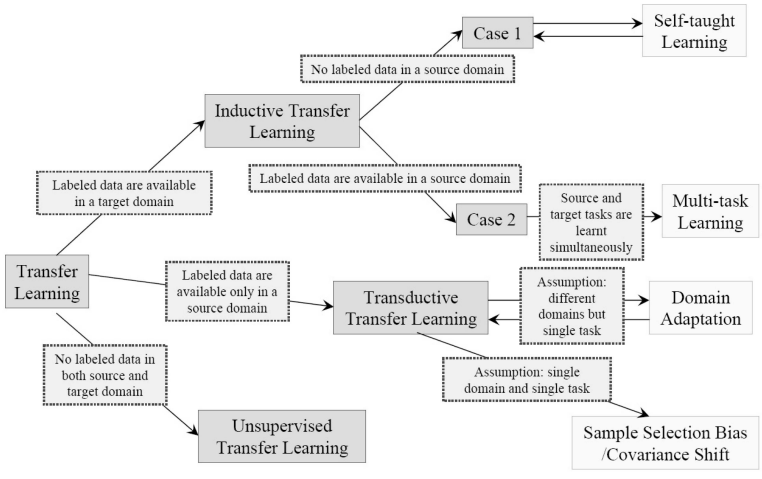
\includegraphics[width=350pt,height=200pt]{pictures/transfer_learning_types.PNG}
  \caption{Overview of the different types of transfer learning.\cite{pan2009survey}}
  \label{fig:transfer_learning_overview}
\end{figure} 

\subsection{Dimensionality Reduction}
Reducing the number of features (i.e. dimensions) in a dataset without sacrificing its relevant attributes is known as dimensionality reduction \cite{deng2022dimensionality}. This is equivalent to eliminating features that are superfluous, redundant or just noisy data, in order to build a model with fewer variables. Dimensionality reduction refers to a variety of preprocessing techniques for feature selection and data compression. Although dimensionality reduction techniques operate differently, they all use variable extraction or combination to convert high-dimensional spaces into low-dimensional spaces.\cite{deng2022dimensionality}

\vspace{5mm}

Dimensions, often known as features or input variables, are predictor variables in machine learning that control a model's output.  Any dataset having a significant number of predictor variables is regarded as high-dimensional data. Machine learning algorithms face several practical challenges when dealing with high-dimensional datasets, including longer calculation times and larger data storage requirements. Perhaps the greatest worry though, is that predictive models are becoming less accurate. Models in machine learning that are trained on high-dimensional datasets frequently have poor generalization.\cite{deng2022dimensionality}

\vspace{5mm}

\textbf{Curse of dimensionality} The inverse link between growing model dimensions and declining generalizability is known as the "curse of dimensionality". The model space rises with the amount of model input variables. Conversely, sparse data results from a constant amount of data points. This indicates that much of the feature space of the model is empty or devoid of observable data points. Data points get so different from one another as data sparsity rises that prediction models are less successful in finding explanatory patterns \cite{Goodfellow-et-al-2016}. Models may overfit on training data in order to explain patterns in sparse data sufficiently. Thus, poor generalizability may result from increases in dimensionality. By causing multicollinearity, high dimensionality might further impede model interpretability \cite{bellman46adaptive}. The effect of the number of model parameters on the performance of the model is shown in Fig. \ref{fig:dimensionality_reduction}.
\begin{figure}[t]
  \centering
  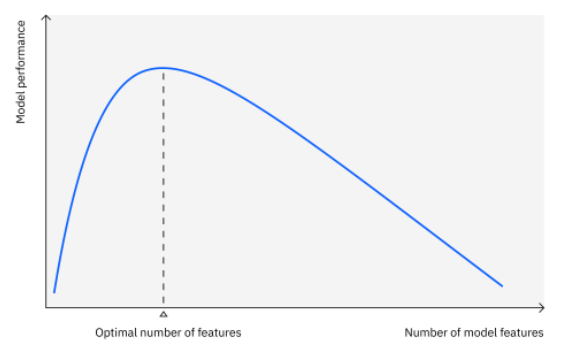
\includegraphics[width=350pt,height=200pt]{pictures/curse_of_dimensionality.PNG}
  \caption{The effect of the number of model parameters on the model performance.\cite{dr}}
  \label{fig:dimensionality_reduction}
\end{figure} 
 There is a chance that certain variables are unnecessary or associated as the number of model variables rises. The curse of dimensionality can be mitigated by increasing the collection of data by reducing data sparsity. However, the number of data points required to counteract the curse of dimensionality grows exponentially with the number of dimensions in a model. Its not always possible of course, to gather enough data. Therefore, dimensionality reduction is necessary to enhance data analysis. \ac{PCA}, \ac{LDA} and \ac{t-SNE} are dimensionality reduction algorithms that improve machine learning models.\cite{deng2022dimensionality}

\subsubsection{Linear Discriminant Analysis}
In supervised machine learning, \ac{LDA} is a method used to resolve multi-class classification problems. It reduces the dimensionality of the data to enable the separation of several classes with numerous features. A generative model framework is used in \ac{LDA}, which is often referred to as \ac{NDA} or \ac{DFA}. In other words, \ac{LDA} algorithms estimate the distribution of data for each class and classify additional data points by applying Bayes' Theorem \cite{bellman46adaptive}. Conditional probabilities or the likelihood of an event given the occurrence of another event are computed by Bayes Theorem. It is used by \ac{LDA} algorithms to determine the likelihood that a particular data item will be included in a specific output. Finding a linear feature combination that distinguishes any number of categories of objects or events is how \ac{LDA} operates. To facilitate easier classification, \ac{LDA} projects data with at least two dimensions into a single dimension as shown in Fig. \ref{fig:lda}. 
\begin{figure}[h]
  \centering
  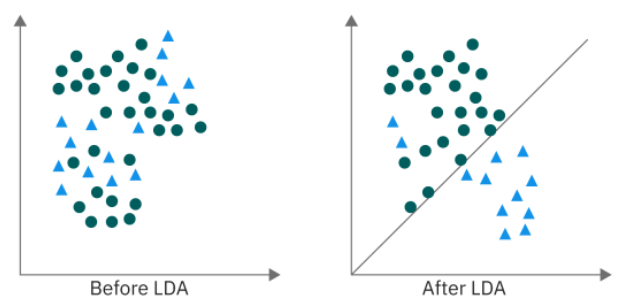
\includegraphics[width=300pt,height=200pt]{pictures/lda.PNG}
  \caption{Projection of the data before and after applying \ac{LDA}.\cite{dr}}
  \label{fig:lda}
\end{figure} 
As a result, the method is occasionally called "dimensionality reduction". Unlike logistic regression for example, which is restricted to binary classification, \ac{LDA}'s adaptability guarantees that it may be applied to multi-class data classification issues. For this reason, it is frequently used to improve the performance of other machine learning classification methods, such as \ac{SVM}, random forests and decision trees.\cite{xanthopoulos2013linear}

\subsubsection{Principal Component Analysis}
Similar to \ac{LDA}, \ac{PCA} is also a dimension reduction method. Unlike \ac{LDA}, it is not restricted to problems involving supervised learning. In other words, PCA can reduce dimensions for unsupervised learning tasks without taking class labels or categories into account. Mathematician Karl Pearson first presented the \ac{PCA} approach in 1901 \cite{sanguansat2012principal}. It functions under the requirement that the variance of the data in the space of fewer dimensions should be maximal even when data in a space with more dimensions is transformed to data in a lower dimensional space as shown in Fig. \ref{fig:pca}. In an unsupervised learning paradigm it can find the correlation between different features in the dataset.
\begin{figure}[t]
  \centering
  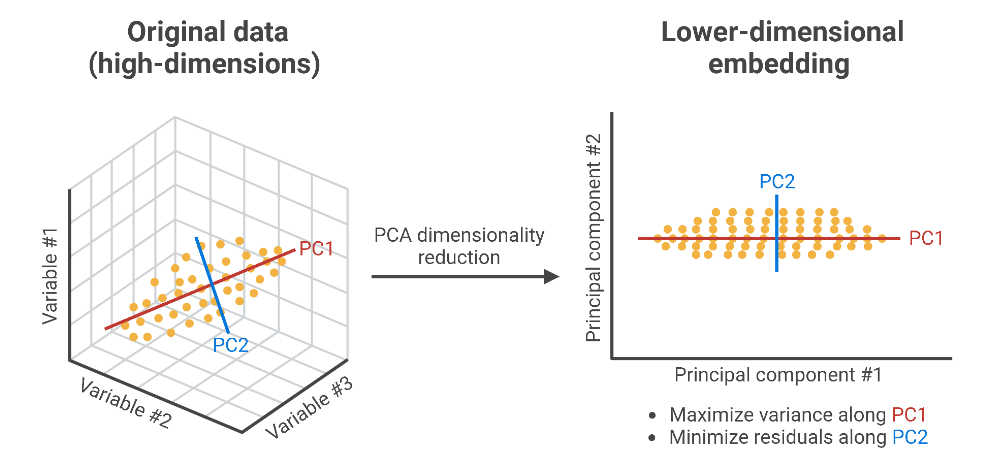
\includegraphics[width=350pt,height=200pt]{pictures/pca.PNG}
  \caption{Projection of the data from higher dimensional space to lower dimensional space on applying \ac{PCA}\cite{pca}}
  \label{fig:pca}
\end{figure} 
A linear combination of the the variables in the original dataset gives rise to the principal components.  By combining the variables in this manner, the majority of the information found in the original variables is condensed into the first components and these new variables or principal components are left uncorrelated. The premise is that ten-dimensional data sets provide ten principal components. PCA then attempts to assign the maximum amount of information to the first principal component, the maximum amount of information left to the second principal component and so on, until the result is somewhat like the Fig. \ref{fig:pca_variables}. By removing the components with little information and using the ones that remain as the new variables, the dimensionality can be minimized without compromising much information when the data is organized using principle components. Its crucial to understand that the primary components are created as linear combinations of the original variables, they are less interpretable and have no true significance. From a geometric perspective, the principal components are the data's directions that account for the greatest amount of variance or the lines that encompass the majority of the data's information. Here, variation and information are related in that a line's variance indicates how dispersed the data points are along it. The more dispersion a line has, the more data it contains. To put all of this into perspective, principle components are new vectors that offer the optimal viewpoint for examining and assessing the data, making the variations between the observations easier to observe.\cite{abdi2010principal} 

\vspace{5mm}

\textbf{Working priniciple for \ac{PCA}}\\
\begin{figure}[t] 
  \centering
  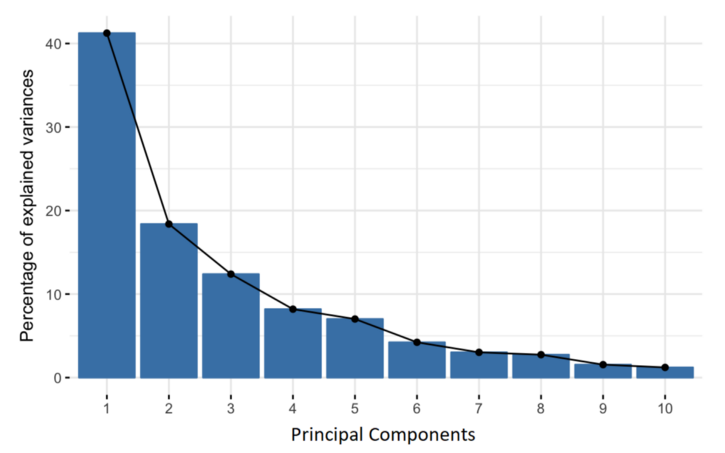
\includegraphics[width=350pt,height=200pt]{pictures/pca_variables.PNG}
  \caption{The percentage of explained variance for each principal component}
  \label{fig:pca_variables}
\end{figure}

\begin{enumerate}
  \item \textbf{Normalization} This step's objective is to normalize the continuous original variable's range to ensure each one makes an equal contribution to the analysis. More precisely, the reason \ac{PCA} is extremely sensitive to the variances of the original variables is because normalization must be done first. In other words, if the ranges of the initial variables differ significantly, the variables with greater ranges will take precedence over the variables with smaller ranges, which will produce biased results. Therefore, this issue can be avoided by translating the data to similar scales. The mathematical procedure for achieving this is to take each variable's value, subtract the mean and then divide the result by the standard deviation as shown in Eq. \ref{eq:norm}.
  \begin{equation}
    \label{eq:norm}
    \mathit{z} = \mathit{\frac{value-mean}{standard deviation}}.
  \end{equation}
  All of these variables will be converted to the same scale after standardization is complete.
  \item \textbf{Computation of covariance matrix} This step's objective is to determine whether there is a correlation between the variables in the dataset being analyzed and how they differ from the mean in relation to one another. Because variables might occasionally include redundant information due to strong correlations, the matrix of covariance is calculated to find these correlations. The correlation matrix of a 3-D data with variables $a$, $b$, $c$ are given by the covariance matrix shown below.\cite{abdi2010principal}
\begin{equation}
  \label{eq:cov_mat}
    \begin{bmatrix}
    Cov(a,a) & Cov(a,b) & Cov(a,c)\\
    Cov(b,a) & Cov(a,b) & Cov(a,c)\\
    Cov(c,a) & Cov(a,b) & Cov(a,c)
  \end{bmatrix}
\end{equation}
  The covariance matrix has all possible pairs of initial variables as entries and is a p × p symmetric matrix (where p is the number of dimensions).
  The variances of each starting variable are along the major diagonal (top left to bottom right), as the variance of a variable with itself is its covariance $(Cov(a,a)=Var(a))$. Furthermore, because the covariance is commutative $(Cov(a,b)=Cov(b,a))$, the covariance matrix's entries are symmetric with regard to the main diagonal, meaning that the top and lower triangular sections are equal. When two variables increase or decrease at the same time, i.e. they are correlated, then the value in the covariance matrix is positive. Whereas, if the two variables doesn't follow the same trend, i.e. one increases while the other decreases, then the variables are uncorrelated.\cite{abdi2010principal}
  \item \textbf{Computation of eigenvectors and eigenvalues} The two necessary mathematical concepts that are essential for the computation of the principal components are eigenvectors and eigenvalues. Every eigenvector has an associated eigenvalue with it. The number of eigenvectors or eigenvalues for the data is equivalent to the dimension of the data. The eigenvector gives the direction of the axis along which most of the variance of the original dataset is preserved or in other words the direction of the principal components. The eigenvalue associated with the eigenvector is the coefficient of the eigenvector, i.e. the amount of variance that particular principal component is responsible for in the total variance. The principal components are obtained by arranging the eigenvectors from highest to lowest of their corresponsing eigenvalues.\cite{abdi2010principal} 
  \item \textbf{Creation of feature vector} Creating the feature vector involves selecting which elements to keep and which to remove. Generally speaking, components with low eigenvalues won't be as important. A plot is generated to display the cumulative proportion of variation as well as the percentage of total variance. Typically, the number of PCA components that is to be included is indicated by the point at which the Y axis of eigenvalues or total variance forms a "elbow".\cite{abdi2010principal}
  \item \textbf{Data transformation along the axis of principal components} With the exception of normalization, none of the data is altered in the preceding steps. Instead, the input data set is always expressed in terms of the original axes or the original variables. The primary components are chosen and the feature vector is created. The goal of this final step is to reorient the data from the original axis to that of the principal components, thus, the name Principal Components Analysis represent by utilizing the feature vector that was created using the eigenvectors of the covariance matrix. To accomplish this, the feature vector's transpose is multiplied by the original data set's transpose as shown in Eq. \ref{eq:trans_data}.\cite{abdi2010principal}
  \begin{equation}
    \label{eq:trans_data}
    \mathit{TransformedDataSet} = \mathit{FeatureVector^T \times NormalizedOriginalDataSet^T}.
  \end{equation}
\end{enumerate}
\cleardoublepage
